% Options for packages loaded elsewhere
% Options for packages loaded elsewhere
\PassOptionsToPackage{unicode}{hyperref}
\PassOptionsToPackage{hyphens}{url}
\PassOptionsToPackage{dvipsnames,svgnames,x11names}{xcolor}
%
\documentclass[
  russian,
  letterpaper,
  DIV=11,
  numbers=noendperiod]{scrartcl}
\usepackage{xcolor}
\usepackage{amsmath,amssymb}
\setcounter{secnumdepth}{5}
\usepackage{iftex}
\ifPDFTeX
  \usepackage[T1]{fontenc}
  \usepackage[utf8]{inputenc}
  \usepackage{textcomp} % provide euro and other symbols
\else % if luatex or xetex
  \usepackage{unicode-math} % this also loads fontspec
  \defaultfontfeatures{Scale=MatchLowercase}
  \defaultfontfeatures[\rmfamily]{Ligatures=TeX,Scale=1}
\fi
\usepackage{lmodern}
\ifPDFTeX\else
  % xetex/luatex font selection
\fi
% Use upquote if available, for straight quotes in verbatim environments
\IfFileExists{upquote.sty}{\usepackage{upquote}}{}
\IfFileExists{microtype.sty}{% use microtype if available
  \usepackage[]{microtype}
  \UseMicrotypeSet[protrusion]{basicmath} % disable protrusion for tt fonts
}{}
\makeatletter
\@ifundefined{KOMAClassName}{% if non-KOMA class
  \IfFileExists{parskip.sty}{%
    \usepackage{parskip}
  }{% else
    \setlength{\parindent}{0pt}
    \setlength{\parskip}{6pt plus 2pt minus 1pt}}
}{% if KOMA class
  \KOMAoptions{parskip=half}}
\makeatother
% Make \paragraph and \subparagraph free-standing
\makeatletter
\ifx\paragraph\undefined\else
  \let\oldparagraph\paragraph
  \renewcommand{\paragraph}{
    \@ifstar
      \xxxParagraphStar
      \xxxParagraphNoStar
  }
  \newcommand{\xxxParagraphStar}[1]{\oldparagraph*{#1}\mbox{}}
  \newcommand{\xxxParagraphNoStar}[1]{\oldparagraph{#1}\mbox{}}
\fi
\ifx\subparagraph\undefined\else
  \let\oldsubparagraph\subparagraph
  \renewcommand{\subparagraph}{
    \@ifstar
      \xxxSubParagraphStar
      \xxxSubParagraphNoStar
  }
  \newcommand{\xxxSubParagraphStar}[1]{\oldsubparagraph*{#1}\mbox{}}
  \newcommand{\xxxSubParagraphNoStar}[1]{\oldsubparagraph{#1}\mbox{}}
\fi
\makeatother


\usepackage{longtable,booktabs,array}
\usepackage{calc} % for calculating minipage widths
% Correct order of tables after \paragraph or \subparagraph
\usepackage{etoolbox}
\makeatletter
\patchcmd\longtable{\par}{\if@noskipsec\mbox{}\fi\par}{}{}
\makeatother
% Allow footnotes in longtable head/foot
\IfFileExists{footnotehyper.sty}{\usepackage{footnotehyper}}{\usepackage{footnote}}
\makesavenoteenv{longtable}
\usepackage{graphicx}
\makeatletter
\newsavebox\pandoc@box
\newcommand*\pandocbounded[1]{% scales image to fit in text height/width
  \sbox\pandoc@box{#1}%
  \Gscale@div\@tempa{\textheight}{\dimexpr\ht\pandoc@box+\dp\pandoc@box\relax}%
  \Gscale@div\@tempb{\linewidth}{\wd\pandoc@box}%
  \ifdim\@tempb\p@<\@tempa\p@\let\@tempa\@tempb\fi% select the smaller of both
  \ifdim\@tempa\p@<\p@\scalebox{\@tempa}{\usebox\pandoc@box}%
  \else\usebox{\pandoc@box}%
  \fi%
}
% Set default figure placement to htbp
\def\fps@figure{htbp}
\makeatother



\ifLuaTeX
\usepackage[bidi=basic,provide=*]{babel}
\else
\usepackage[bidi=default,provide=*]{babel}
\fi
% get rid of language-specific shorthands (see #6817):
\let\LanguageShortHands\languageshorthands
\def\languageshorthands#1{}


\setlength{\emergencystretch}{3em} % prevent overfull lines

\providecommand{\tightlist}{%
  \setlength{\itemsep}{0pt}\setlength{\parskip}{0pt}}



 


\usepackage{fontspec}

\setsansfont{Palatino Linotype}[
    Path=../files/palatino/,
    Extension = .ttf,
    UprightFont=palatino-Roman,
    BoldFont=palatino-Bold,
    ItalicFont=palatino-Italic,
    BoldItalicFont=palatino-BoldItalic
]
\setmainfont{Palatino Linotype}[
    Path=../files/palatino/,
    Extension = .ttf,
    UprightFont=palatino-Roman,
    BoldFont=palatino-Bold,
    ItalicFont=palatino-Italic,
    BoldItalicFont=palatino-BoldItalic
]

\usepackage[textwidth=0.86\paperwidth, textheight=0.86\paperheight]{geometry}
\usepackage{fancyhdr}
\usepackage{hyperref}
\usepackage{fontawesome5}
\usepackage{graphicx}
\usepackage{amssymb}
\usepackage{amsmath}
\graphicspath{{../files/}}

\newcommand{\R}{\mathbb{R}}

% \pagenumbering{gobble}
\pagestyle{fancy}
\fancyhead{} % clear all header fields
\fancyhead[R]{\href{https://cu25.fmin.xyz}{\faGem[regular]} \hspace{0.04cm} \href{https://github.com/MerkulovDaniil/cu25}{\faGithub} \hspace{0.07cm} \href{https://t.me/fminxyz}{\faTelegram}}
\fancyhead[L]{\href{https://fmin.xyz}{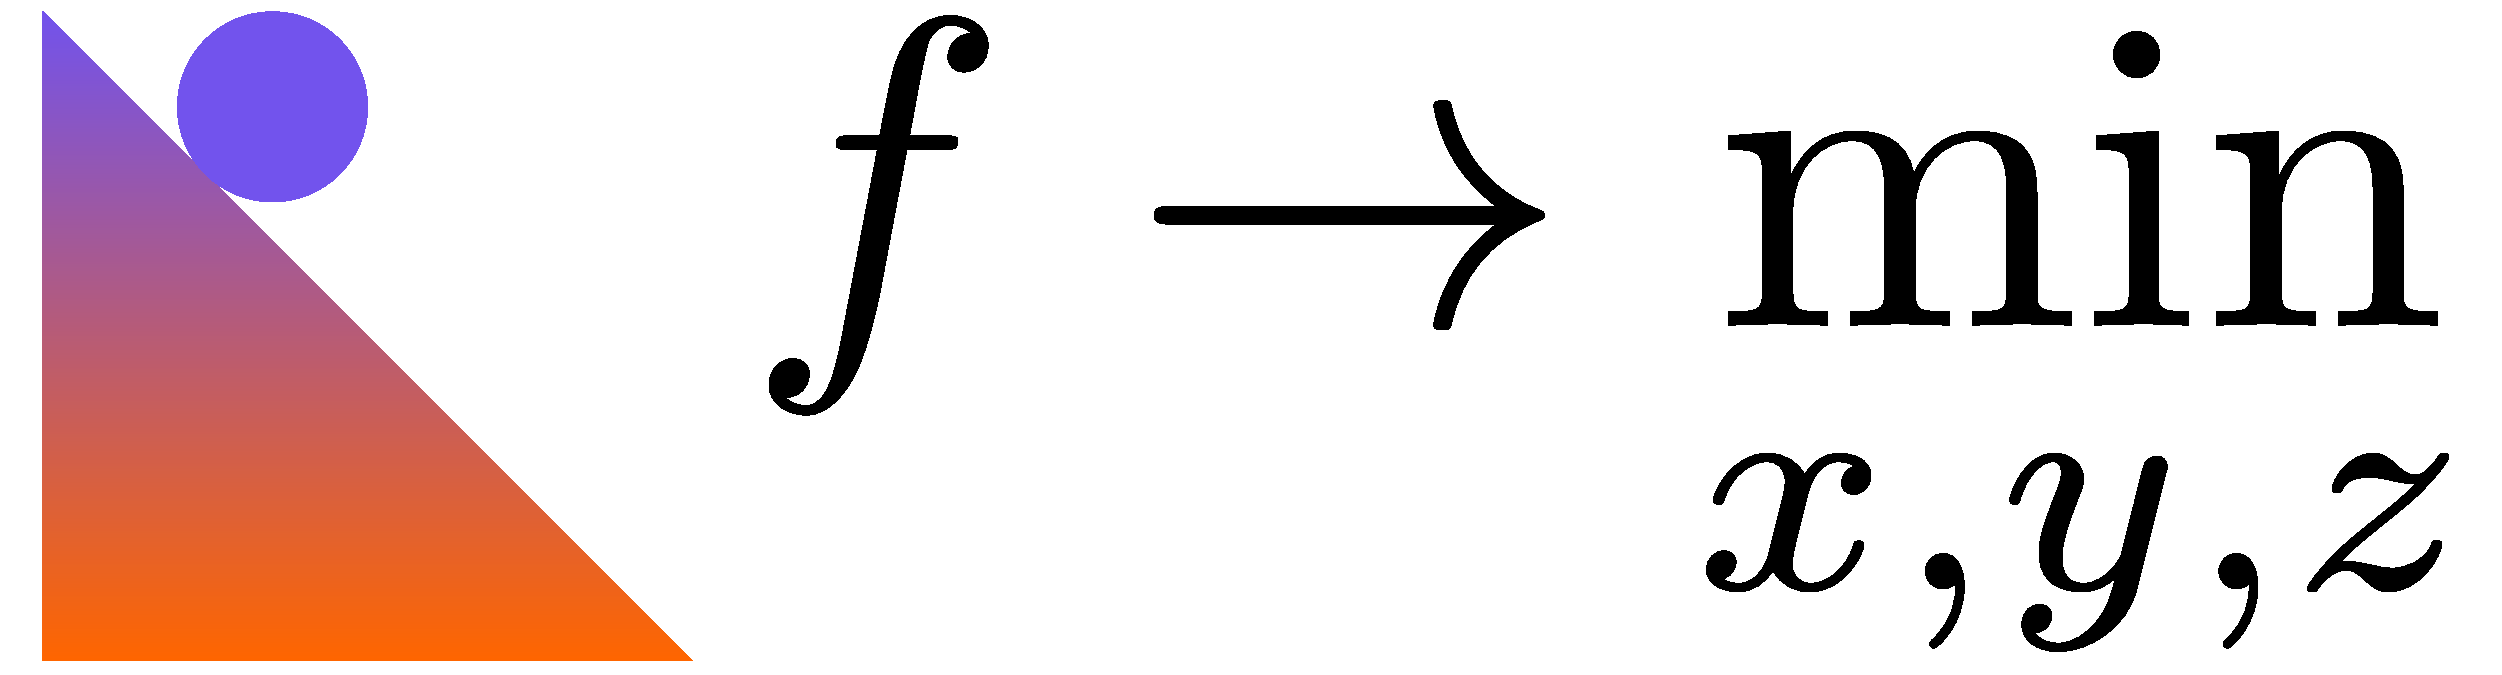
\includegraphics[height=0.35cm]{logo.pdf}} \hspace{2pt} \textbf{Оптимизация для всех! ЦУ. 2025}}
\KOMAoption{captions}{tableheading}
\makeatletter
\@ifpackageloaded{tcolorbox}{}{\usepackage[skins,breakable]{tcolorbox}}
\@ifpackageloaded{fontawesome5}{}{\usepackage{fontawesome5}}
\definecolor{quarto-callout-color}{HTML}{909090}
\definecolor{quarto-callout-note-color}{HTML}{0758E5}
\definecolor{quarto-callout-important-color}{HTML}{CC1914}
\definecolor{quarto-callout-warning-color}{HTML}{EB9113}
\definecolor{quarto-callout-tip-color}{HTML}{00A047}
\definecolor{quarto-callout-caution-color}{HTML}{FC5300}
\definecolor{quarto-callout-color-frame}{HTML}{acacac}
\definecolor{quarto-callout-note-color-frame}{HTML}{4582ec}
\definecolor{quarto-callout-important-color-frame}{HTML}{d9534f}
\definecolor{quarto-callout-warning-color-frame}{HTML}{f0ad4e}
\definecolor{quarto-callout-tip-color-frame}{HTML}{02b875}
\definecolor{quarto-callout-caution-color-frame}{HTML}{fd7e14}
\makeatother
\makeatletter
\@ifpackageloaded{caption}{}{\usepackage{caption}}
\AtBeginDocument{%
\ifdefined\contentsname
  \renewcommand*\contentsname{Содержание}
\else
  \newcommand\contentsname{Содержание}
\fi
\ifdefined\listfigurename
  \renewcommand*\listfigurename{Список Иллюстраций}
\else
  \newcommand\listfigurename{Список Иллюстраций}
\fi
\ifdefined\listtablename
  \renewcommand*\listtablename{Список Таблиц}
\else
  \newcommand\listtablename{Список Таблиц}
\fi
\ifdefined\figurename
  \renewcommand*\figurename{Рисунок}
\else
  \newcommand\figurename{Рисунок}
\fi
\ifdefined\tablename
  \renewcommand*\tablename{Таблица}
\else
  \newcommand\tablename{Таблица}
\fi
}
\@ifpackageloaded{float}{}{\usepackage{float}}
\floatstyle{ruled}
\@ifundefined{c@chapter}{\newfloat{codelisting}{h}{lop}}{\newfloat{codelisting}{h}{lop}[chapter]}
\floatname{codelisting}{Список}
\newcommand*\listoflistings{\listof{codelisting}{Список Каталогов}}
\makeatother
\makeatletter
\makeatother
\makeatletter
\@ifpackageloaded{caption}{}{\usepackage{caption}}
\@ifpackageloaded{subcaption}{}{\usepackage{subcaption}}
\makeatother
\usepackage{bookmark}
\IfFileExists{xurl.sty}{\usepackage{xurl}}{} % add URL line breaks if available
\urlstyle{same}
\hypersetup{
  pdftitle={Выпуклость: выпуклые множества, выпуклые функции. Условие Поляка - Лоясиевича. Сильная выпуклость},
  pdfauthor={Даня Меркулов},
  pdflang={ru},
  colorlinks=true,
  linkcolor={blue},
  filecolor={Maroon},
  citecolor={Blue},
  urlcolor={Blue},
  pdfcreator={LaTeX via pandoc}}


\title{Выпуклость: выпуклые множества, выпуклые функции. Условие Поляка
- Лоясиевича. Сильная выпуклость}
\author{Даня Меркулов}
\date{}
\begin{document}
\maketitle


\section{Выпуклые
множества}\label{ux432ux44bux43fux443ux43aux43bux44bux435-ux43cux43dux43eux436ux435ux441ux442ux432ux430}

\subsection{Аффинные
множества}\label{ux430ux444ux444ux438ux43dux43dux44bux435-ux43cux43dux43eux436ux435ux441ux442ux432ux430}

Пусть \(x_1, x_2\) два вектора в \(\mathbb{R}^n\). Тогда прямая,
проходящая через них, определяется следующим образом: \[
x = \theta x_1 + (1 - \theta)x_2, \theta \in \mathbb{R}
\] Множество \(A\) называется \textbf{аффинным}, если для любых
\(x_1, x_2\) из \(A\) прямая, проходящая через них, также лежит в \(A\),
т.е. \[
\forall \theta \in \mathbb{R}, \forall x_1, x_2 \in A: \theta x_1 + (1- \theta) x_2 \in A
\]

\begin{tcolorbox}[enhanced jigsaw, colframe=quarto-callout-color-frame, titlerule=0mm, coltitle=black, toprule=.15mm, colback=white, leftrule=.75mm, bottomtitle=1mm, toptitle=1mm, colbacktitle=quarto-callout-color!10!white, breakable, opacityback=0, bottomrule=.15mm, left=2mm, opacitybacktitle=0.6, title=\textcolor{quarto-callout-color}{\faInfo}\hspace{0.5em}{Example}, rightrule=.15mm, arc=.35mm]

\begin{itemize}
\tightlist
\item
  \(\mathbb{R}^n\) - аффинное множество.
\item
  Множество решений \(\left\{x \mid \mathbf{A}x =  \mathbf{b} \right\}\)
  также является аффинным множеством.
\end{itemize}

\end{tcolorbox}

\begin{figure}[H]

{\centering \pandocbounded{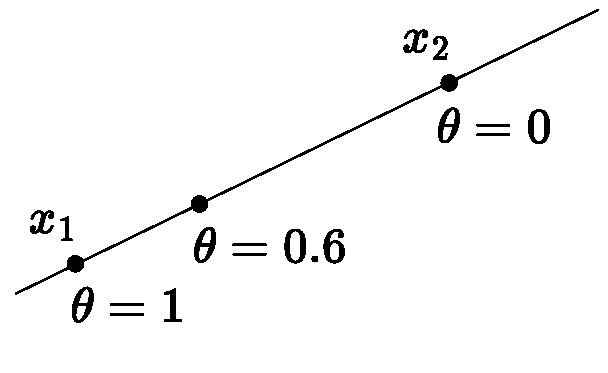
\includegraphics[keepaspectratio]{line.pdf}}

}

\caption{Иллюстрация прямой между двумя векторами \(x_1\) и \(x_2\)}

\end{figure}%

\subsection{Конус}\label{ux43aux43eux43dux443ux441}

Множество \(S\) называется \textbf{конусом}, если: \[
\forall x \in S, \; \theta \ge 0 \;\; \rightarrow \;\; \theta x \in S
\] Если точка принадлежит конусу, то и весь луч, проходящий из начала
координат через эту точку, также принадлежит этому конусу.

\begin{figure}[H]

{\centering \pandocbounded{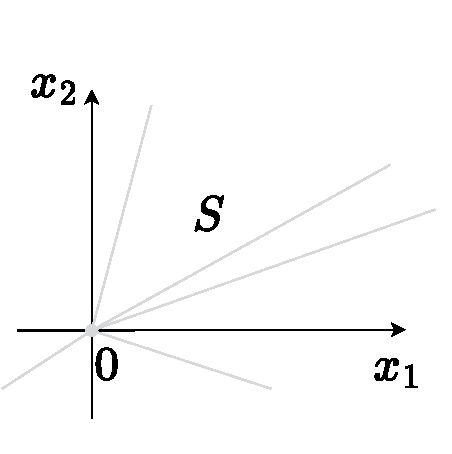
\includegraphics[keepaspectratio]{cone.pdf}}

}

\caption{Иллюстрация конуса}

\end{figure}%

\subsection{Выпуклый
конус}\label{ux432ux44bux43fux443ux43aux43bux44bux439-ux43aux43eux43dux443ux441}

Множество \(S\) называется \textbf{выпуклым конусом}, если: \[
\forall x_1, x_2 \in S, \; \theta_1, \theta_2 \ge 0 \;\; \rightarrow \;\; \theta_1 x_1 + \theta_2 x_2 \in S
\] Выпуклый конус это конус, который также является выпуклым множеством.

\begin{tcolorbox}[enhanced jigsaw, colframe=quarto-callout-color-frame, titlerule=0mm, coltitle=black, toprule=.15mm, colback=white, leftrule=.75mm, bottomtitle=1mm, toptitle=1mm, colbacktitle=quarto-callout-color!10!white, breakable, opacityback=0, bottomrule=.15mm, left=2mm, opacitybacktitle=0.6, title=\textcolor{quarto-callout-color}{\faInfo}\hspace{0.5em}{Example}, rightrule=.15mm, arc=.35mm]

\begin{itemize}
\tightlist
\item
  \(\mathbb{R}^n\)
\item
  Аффинные множества, содержащие \(0\)
\item
  Луч
\item
  \(\mathbf{S}^n_+\) - множество симметричных положительно
  полуопределенных матриц
\end{itemize}

\end{tcolorbox}

Выпуклый конус является выпуклым множеством, содержащим все конические
комбинации точек в множестве.

\begin{figure}[H]

{\centering \pandocbounded{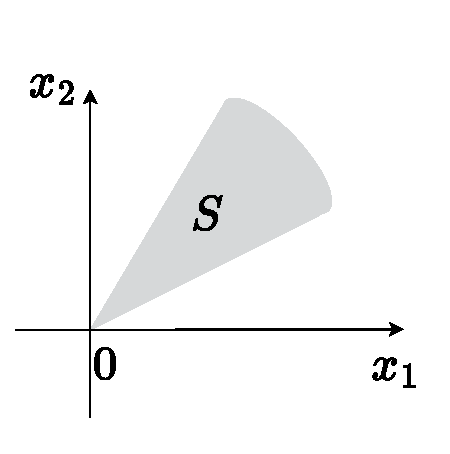
\includegraphics[keepaspectratio]{convex_cone.pdf}}

}

\caption{Иллюстрация выпуклого конуса}

\end{figure}%

\subsection{Отрезок}\label{ux43eux442ux440ux435ux437ux43eux43a}

Пусть \(x_1, x_2\) два вектора в \(\mathbb{R}^n\).

Тогда отрезок между ними определяется следующим образом: \[
x = \theta x_1 + (1 - \theta)x_2, \; \theta \in [0,1]
\] Выпуклое множество содержит отрезок между любыми двумя точками в
множестве.

\begin{figure}[H]

{\centering 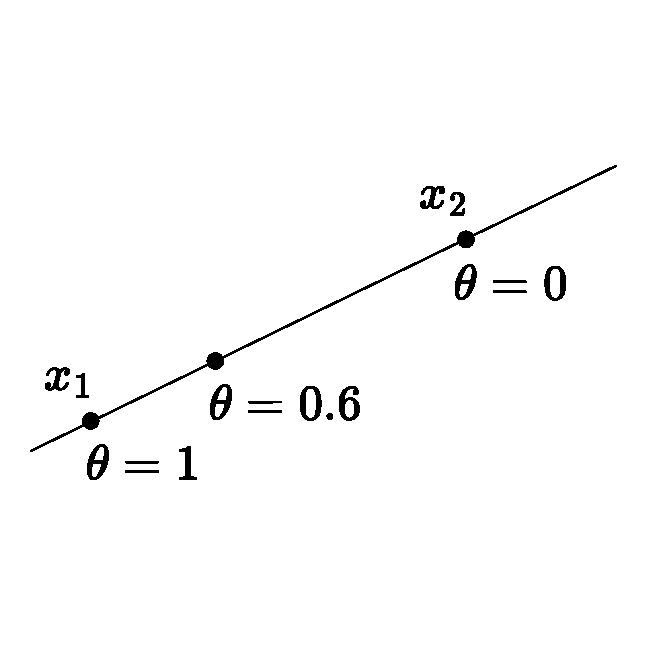
\includegraphics[width=0.5\linewidth,height=\textheight,keepaspectratio]{line_segment.pdf}

}

\caption{Иллюстрация отрезка между точками \(x_1\), \(x_2\)}

\end{figure}%

\subsection{Выпуклое
множество}\label{ux432ux44bux43fux443ux43aux43bux43eux435-ux43cux43dux43eux436ux435ux441ux442ux432ux43e}

Множество \(S\) называется \textbf{выпуклым}, если для любых
\(x_1, x_2\) из \(S\) отрезок между ними также лежит в \(S\), т.е. \[
\forall \theta \in [0,1], \; \forall x_1, x_2 \in S: \theta x_1 + (1- \theta) x_2 \in S
\]

\begin{figure}[H]

{\centering \pandocbounded{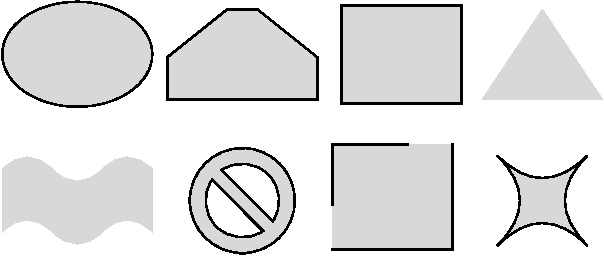
\includegraphics[keepaspectratio]{convex_sets.pdf}}

}

\caption{Верх: примеры выпуклых множеств. Низ: примеры невыпуклых
множеств.}

\end{figure}%

\begin{tcolorbox}[enhanced jigsaw, colframe=quarto-callout-color-frame, titlerule=0mm, coltitle=black, toprule=.15mm, colback=white, leftrule=.75mm, bottomtitle=1mm, toptitle=1mm, colbacktitle=quarto-callout-color!10!white, breakable, opacityback=0, bottomrule=.15mm, left=2mm, opacitybacktitle=0.6, title=\textcolor{quarto-callout-color}{\faInfo}\hspace{0.5em}{Example}, rightrule=.15mm, arc=.35mm]

Пустое множество и множество из одного вектора являются выпуклыми по
определению.

\end{tcolorbox}

\begin{tcolorbox}[enhanced jigsaw, colframe=quarto-callout-color-frame, titlerule=0mm, coltitle=black, toprule=.15mm, colback=white, leftrule=.75mm, bottomtitle=1mm, toptitle=1mm, colbacktitle=quarto-callout-color!10!white, breakable, opacityback=0, bottomrule=.15mm, left=2mm, opacitybacktitle=0.6, title=\textcolor{quarto-callout-color}{\faInfo}\hspace{0.5em}{Example}, rightrule=.15mm, arc=.35mm]

Любое аффинное множество, луч или отрезок являются выпуклыми
множествами.

\end{tcolorbox}

\subsection{Выпуклая
комбинация}\label{ux432ux44bux43fux443ux43aux43bux430ux44f-ux43aux43eux43cux431ux438ux43dux430ux446ux438ux44f}

Пусть \(x_1, x_2, \ldots, x_k \in S\), тогда точка
\(\theta_1 x_1 + \theta_2 x_2 + \ldots + \theta_k x_k\) называется
\textbf{выпуклой комбинацией} точек \(x_1, x_2, \ldots, x_k\) если
\(\sum\limits_{i=1}^k\theta_i = 1, \; \theta_i \ge 0\).

\subsection{Выпуклая
оболочка}\label{ux432ux44bux43fux443ux43aux43bux430ux44f-ux43eux431ux43eux43bux43eux447ux43aux430}

Множество всех выпуклых комбинаций точек из \(S\) называется
\textbf{выпуклой оболочкой} множества \(S\). \[
\mathbf{conv}(S) = \left\{ \sum\limits_{i=1}^k\theta_i x_i \mid x_i \in S, \sum\limits_{i=1}^k\theta_i = 1, \; \theta_i \ge 0\right\}
\] * Множество \(\mathbf{conv}(S)\) является наименьшим выпуклым
множеством, содержащим \(S\). * Множество \(S\) является выпуклым тогда
и только тогда, когда \(S = \mathbf{conv}(S)\).

\begin{figure}[H]

{\centering \pandocbounded{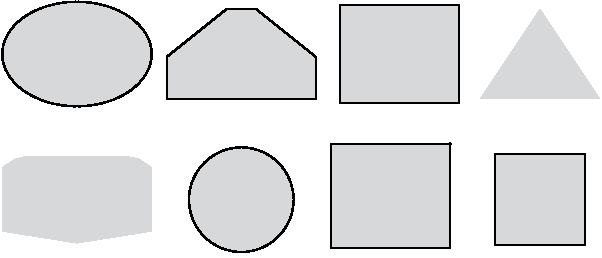
\includegraphics[keepaspectratio]{convex_hulls.pdf}}

}

\caption{Верх: выпуклые оболочки выпуклых множеств. Низ: выпуклая
оболочка невыпуклых множеств.}

\end{figure}%

\subsection{Сумма
Минковского}\label{ux441ux443ux43cux43cux430-ux43cux438ux43dux43aux43eux432ux441ux43aux43eux433ux43e}

Сумма Минковского двух множеств векторов \(S_1\) и \(S_2\) в евклидовом
пространстве образуется путем сложения каждого вектора из \(S_1\) с
каждым вектором из \(S_2\). \[
S_1+S_2=\{\mathbf {s_1} +\mathbf {s_2} \,|\,\mathbf {s_1} \in S_1,\ \mathbf {s_2} \in S_2\}
\] Также можно определить линейную комбинацию множеств.

\begin{tcolorbox}[enhanced jigsaw, colframe=quarto-callout-color-frame, titlerule=0mm, coltitle=black, toprule=.15mm, colback=white, leftrule=.75mm, bottomtitle=1mm, toptitle=1mm, colbacktitle=quarto-callout-color!10!white, breakable, opacityback=0, bottomrule=.15mm, left=2mm, opacitybacktitle=0.6, title=\textcolor{quarto-callout-color}{\faInfo}\hspace{0.5em}{Example}, rightrule=.15mm, arc=.35mm]

Рассмотрим пространство \(\mathbb{R}^2\). Определим: \[
S_1 := \{x \in \mathbb{R}^2 : x_1^2 + x_2^2 \leq 1\}
\] Это единичная окружность, с центром в начале координат. И: \[
S_2 := \{x \in \mathbb{R}^2 : -4 \leq x_1 \leq -1, -3 \leq x_2 \leq -1\}
\]

Это прямоугольник. Сумма множеств \(S_1\) и \(S_2\) образуетувеличенный
прямоугольник \(S_2\) с закругленными углами. Полученное множество будет
выпуклым.

\begin{figure}[H]

{\centering 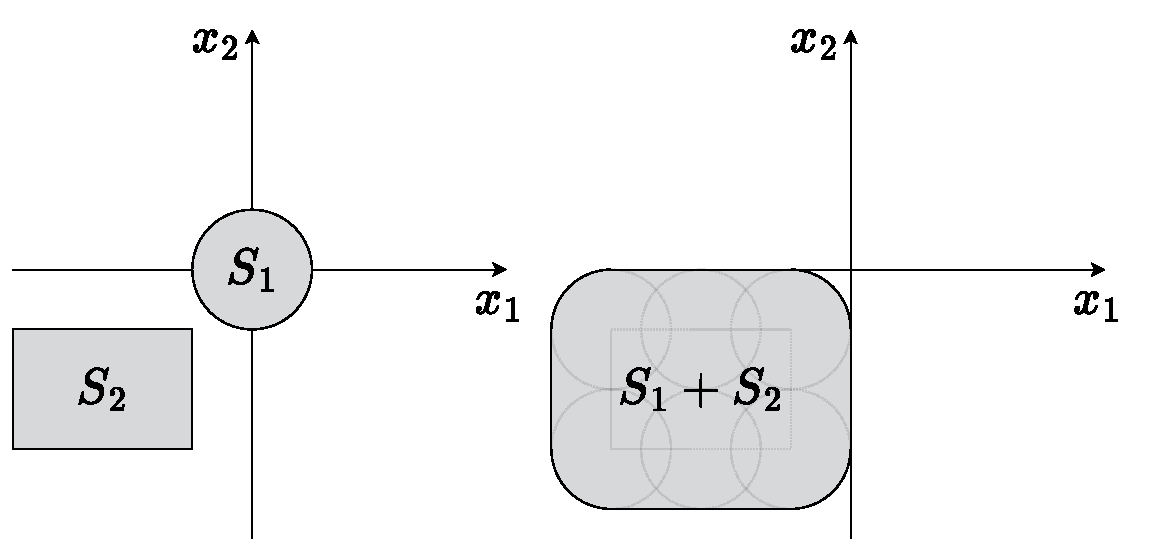
\includegraphics[width=0.7\linewidth,height=\textheight,keepaspectratio]{minkowski.pdf}

}

\caption{\(S = S_1 + S_2\)}

\end{figure}%

\end{tcolorbox}

\subsection{Проверка
выпуклости}\label{ux43fux440ux43eux432ux435ux440ux43aux430-ux432ux44bux43fux443ux43aux43bux43eux441ux442ux438}

На практике очень важно понимать, является ли конкретное множество
выпуклым или нет. Для этого используются два подхода в зависимости от
контекста.

\begin{itemize}
\tightlist
\item
  По определению.
\item
  Показать, что \(S\) получается из простых выпуклых множеств с помощью
  операций, сохраняющих выпуклость.
\end{itemize}

\subsection{Проверка выпуклости по
определению}\label{ux43fux440ux43eux432ux435ux440ux43aux430-ux432ux44bux43fux443ux43aux43bux43eux441ux442ux438-ux43fux43e-ux43eux43fux440ux435ux434ux435ux43bux435ux43dux438ux44e}

\[
x_1, x_2 \in S, \; 0 \le \theta \le 1 \;\; \rightarrow \;\; \theta x_1 + (1-\theta)x_2 \in S
\]

\begin{tcolorbox}[enhanced jigsaw, colframe=quarto-callout-color-frame, titlerule=0mm, coltitle=black, toprule=.15mm, colback=white, leftrule=.75mm, bottomtitle=1mm, toptitle=1mm, colbacktitle=quarto-callout-color!10!white, breakable, opacityback=0, bottomrule=.15mm, left=2mm, opacitybacktitle=0.6, title=\textcolor{quarto-callout-color}{\faInfo}\hspace{0.5em}{Example}, rightrule=.15mm, arc=.35mm]

Доказать, что множество симметричных положительно определенных матриц
\(\mathbf{S}^n_{++} = \{ \mathbf{X} \in \mathbb{R}^{n \times n} \mid \mathbf{X} = \mathbf{X}^\top, \; \mathbf{X} \succ 0 \}\)
является выпуклым.

\end{tcolorbox}

\subsection{Операции, сохраняющие
выпуклость}\label{ux43eux43fux435ux440ux430ux446ux438ux438-ux441ux43eux445ux440ux430ux43dux44fux44eux449ux438ux435-ux432ux44bux43fux443ux43aux43bux43eux441ux442ux44c}

Линейная комбинация выпуклых множеств является выпуклым множеством.

Пусть есть два выпуклых множества \(S_x, S_y\), тогда множество \[
S = \left\{s \mid s = c_1 x + c_2 y, \; x \in S_x, \; y \in S_y, \; c_1, c_2 \in \mathbb{R}\right\}
\] Возьмем два вектора из \(S\):
\(s_1 = c_1 x_1 + c_2 y_1, s_2 = c_1 x_2 + c_2 y_2\) и докажем, что
отрезок между ними \(\theta  s_1 + (1 - \theta)s_2, \theta \in [0,1]\)
также принадлежит \(S\) \[
\theta s_1 + (1 - \theta)s_2
\] \[
\theta (c_1 x_1 + c_2 y_1) + (1 - \theta)(c_1 x_2 + c_2 y_2)
\] \[
c_1 (\theta x_1 + (1 - \theta)x_2) + c_2 (\theta y_1 + (1 - \theta)y_2)
\] \[
c_1 x + c_2 y \in S
\]

\subsection{Пересечение любого (!) числа выпуклых множеств является
выпуклым}\label{ux43fux435ux440ux435ux441ux435ux447ux435ux43dux438ux435-ux43bux44eux431ux43eux433ux43e-ux447ux438ux441ux43bux430-ux432ux44bux43fux443ux43aux43bux44bux445-ux43cux43dux43eux436ux435ux441ux442ux432-ux44fux432ux43bux44fux435ux442ux441ux44f-ux432ux44bux43fux443ux43aux43bux44bux43c}

Если пересечение пустое или содержит одну точку, свойство доказывается
по определению. В противном случае возьмем две точки и отрезок между
ними. Эти точки должны лежать во всех пересекающихся множествах, и
поскольку они все выпуклые, отрезок между ними лежит во всех множествах
и, следовательно, в их пересечении.

\begin{figure}[H]

{\centering 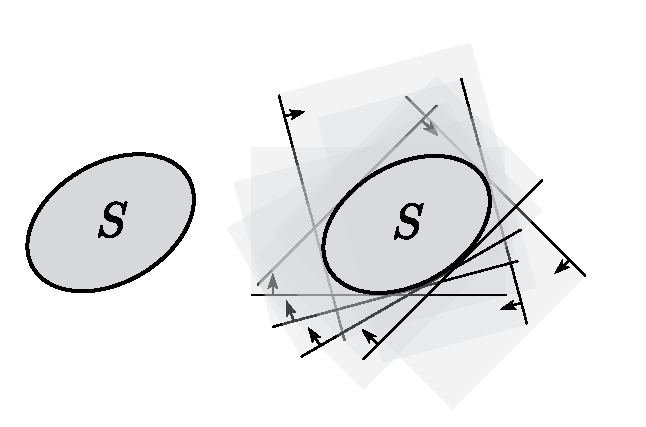
\includegraphics[width=0.5\linewidth,height=\textheight,keepaspectratio]{conv_inter.pdf}

}

\caption{Пересечение полуплоскостей}

\end{figure}%

\subsection{Образ выпуклого множества при аффинном отображении является
выпуклым}\label{ux43eux431ux440ux430ux437-ux432ux44bux43fux443ux43aux43bux43eux433ux43e-ux43cux43dux43eux436ux435ux441ux442ux432ux430-ux43fux440ux438-ux430ux444ux444ux438ux43dux43dux43eux43c-ux43eux442ux43eux431ux440ux430ux436ux435ux43dux438ux438-ux44fux432ux43bux44fux435ux442ux441ux44f-ux432ux44bux43fux443ux43aux43bux44bux43c}

\[
S \subseteq \mathbb{R}^n \text{ выпукло}\;\; \rightarrow \;\; f(S) = \left\{ f(x) \mid x \in S \right\} \text{ выпукло} \;\;\;\; \left(f(x) = \mathbf{A}x + \mathbf{b}\right)
\] Примеры аффинных множеств: расширение, проекция, транспонирование,
множество решений линейного матричного неравенства
\(\left\{ x \mid x_1 A_1 + \ldots + x_m A_m \preceq B\right\}\). Здесь
\(A_i, B \in \mathbf{S}^p\) симметричные матрицы \(p \times p\).

Также обратим внимание, что прообраз выпуклого множества при аффинном
отображении также является выпуклым. \[
S \subseteq \mathbb{R}^m \text{ выпукло}\; \rightarrow \; f^{-1}(S) = \left\{ x \in \mathbb{R}^n \mid f(x) \in S \right\} \text{ выпукло} \;\; \left(f(x) = \mathbf{A}x + \mathbf{b}\right)
\]

\textbf{Пример}

Пусть \(x \in \mathbb{R}\) - случайная величина с заданным вероятностным
распределением \(\mathbb{P}(x = a_i) = p_i\), где \(i = 1, \ldots, n\),
и \(a_1 < \ldots < a_n\). Тогда вектор вероятностей
\(p \in \mathbb{R}^n\) принадлежит вероятностному симплексу, т.е. \[
P = \{ p \mid \mathbf{1}^Tp = 1, p \succeq 0 \} = \{ p \mid p_1 + \ldots + p_n = 1, p_i \ge 0 \}.
\] Определить, являются ли следующие множества вероятностных векторов
\(p\) выпуклыми:

\begin{itemize}
\tightlist
\item
  \(\mathbb{P}(x > \alpha) \le \beta\)
\item
  \(\mathbb{E} \vert x^{201}\vert \le \alpha \mathbb{E}\vert x \vert\)
\item
  \(\mathbb{E} \vert x^{2}\vert \ge \alpha\)\(\mathbb{V} x \ge \alpha\)
\end{itemize}

\section{Выпуклые
функции}\label{ux432ux44bux43fux443ux43aux43bux44bux435-ux444ux443ux43dux43aux446ux438ux438}

\subsection{Неравенство
Йенсена}\label{ux43dux435ux440ux430ux432ux435ux43dux441ux442ux432ux43e-ux439ux435ux43dux441ux435ux43dux430}

Функция \(f(x)\), \textbf{определенная на выпуклом множестве}
\(S \subseteq \mathbb{R}^n\), называется \textbf{выпуклой} на \(S\),
если: \[
f(\lambda x_1 + (1 - \lambda)x_2) \le \lambda f(x_1) + (1 - \lambda)f(x_2)
\] для любых \(x_1, x_2 \in S\) и \(0 \le \lambda \le 1\).\\
Если вышеуказанное неравенство выполняется строгим неравенством для
\(x_1 \neq x_2\) и \(0 < \lambda < 1\), то функция называется строго
выпуклой на \(S\).

\begin{figure}[H]

{\centering \pandocbounded{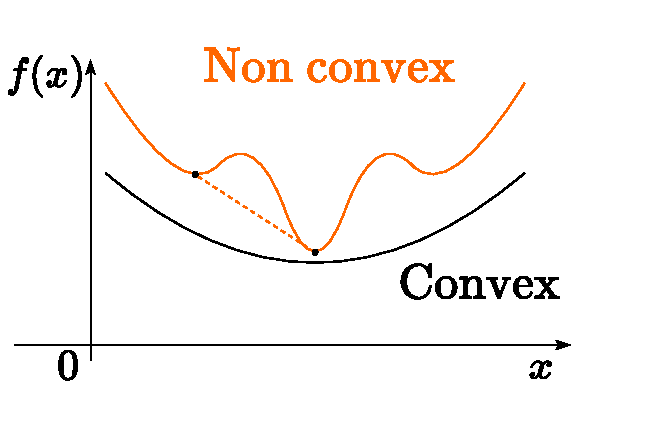
\includegraphics[keepaspectratio]{convex_function.pdf}}

}

\caption{Разница между выпуклой и невыпуклой функцией}

\end{figure}%

\begin{tcolorbox}[enhanced jigsaw, colframe=quarto-callout-color-frame, titlerule=0mm, coltitle=black, toprule=.15mm, colback=white, leftrule=.75mm, bottomtitle=1mm, toptitle=1mm, colbacktitle=quarto-callout-color!10!white, breakable, opacityback=0, bottomrule=.15mm, left=2mm, opacitybacktitle=0.6, title=\textcolor{quarto-callout-color}{\faInfo}\hspace{0.5em}{Theorem}, rightrule=.15mm, arc=.35mm]

Пусть \(f(x)\) выпуклая функция на выпуклом множестве
\(X \subseteq \mathbb{R}^n\) и пусть \(x_i \in X, 1 \leq i \leq m\),
произвольные точки из \(X\). Тогда \[
f\left( \sum_{i=1}^{m} \lambda_i x_i \right) \leq \sum_{i=1}^{m} \lambda_i f(x_i)
\] для любого \(\lambda = [\lambda_1, \ldots, \lambda_m] \in \Delta_m\)
- вероятностного симплекса.

\end{tcolorbox}

\textbf{Доказательство}

\begin{enumerate}
\def\labelenumi{\arabic{enumi}.}
\item
  Во-первых, обратим внимание, что точка
  \(\sum_{i=1}^{m} \lambda_i x_i\) как выпуклая комбинация точек из
  выпуклого множества \(X\) принадлежит \(X\).
\item
  Мы докажем это индукцией. Для \(m = 1\), утверждение очевидно, и для
  \(m = 2\), оно следует из определения выпуклой функции.
\item
  Предположим, что оно верно для всех \(m\) до \(m = k\), и мы докажем
  его для \(m = k + 1\). Пусть \(\lambda \in \Delta{k+1}\) и \[
  x = \sum_{i=1}^{k+1} \lambda_i x_i = \sum_{i=1}^{k} \lambda_i x_i + \lambda_{k+1} x_{k+1}.
  \] Предположим, что \(0 < \lambda_{k+1} < 1\), иначе, оно сводится к
  рассмотренным ранее случаям, тогда мы имеем \[
  x = \lambda_{k+1} x_{k+1} + (1 - \lambda_{k+1}) \bar{x}, 
  \] где \(\bar{x} = \sum_{i=1}^{k} \gamma_i x_i\) и
  \(\gamma_i = \frac{\lambda_i}{1-\lambda_{k+1}} \geq 0, 1 \leq i \leq k\).
\item
  Поскольку \(\lambda \in \Delta_{k+1}\), то
  \(\gamma = [\gamma_1, \ldots, \gamma_k] \in \Delta_k\). Следовательно,
  \(\bar{x} \in X\) и по выпуклости \(f(x)\) и гипотезе индукции: \[
  f\left( \sum_{i=1}^{k+1} \lambda_i x_i \right) = f\left( \lambda_{k+1} x_{k+1} + (1 - \lambda_{k+1})\bar{x} \right) \leq
  \lambda_{k+1}f(x_{k+1}) + (1 - \lambda_{k+1})f(\bar{x}) \leq \sum_{i=1}^{k+1} \lambda_i f(x_i)
  \] Таким образом, исходное неравенство выполняется для \(m = k + 1\).
\end{enumerate}

\textbf{Примеры выпуклых функций}

\begin{itemize}
\tightlist
\item
  \(f(x) = x^p, \;  p > 1,\;  x \in \mathbb{R}_+\)
\item
  \(f(x) = \|x\|^p,\;  p > 1, x \in \mathbb{R}^n\)
\item
  \(f(x) = e^{cx},\;  c \in \mathbb{R}, x \in \mathbb{R}\)
\item
  \(f(x) = -\ln x,\;  x \in \mathbb{R}_{++}\)
\item
  \(f(x) = x\ln x,\;  x \in \mathbb{R}_{++}\)
\item
  Сумма \(k\) наибольших координат
  \(f(x) = x_{(1)} + \ldots + x_{(k)},\; x \in \mathbb{R}^n\)
\item
  \(f(X) = \lambda_{max}(X),\;  X = X^T\)
\item
  \(f(X) = - \log \det X, \;  X \in S^n_{++}\)
\end{itemize}

\subsection{Надграфик}\label{ux43dux430ux434ux433ux440ux430ux444ux438ux43a}

Для функции \(f(x)\), определенной на \(S \subseteq \mathbb{R}^n\),
множество: \[
\text{epi } f = \left\{[x,\mu] \in S \times \mathbb{R}: f(x) \le \mu\right\}
\] называется \textbf{надграфиком} функции \(f(x)\).

\begin{tcolorbox}[enhanced jigsaw, colframe=quarto-callout-color-frame, titlerule=0mm, coltitle=black, toprule=.15mm, colback=white, leftrule=.75mm, bottomtitle=1mm, toptitle=1mm, colbacktitle=quarto-callout-color!10!white, breakable, opacityback=0, bottomrule=.15mm, left=2mm, opacitybacktitle=0.6, title=\textcolor{quarto-callout-color}{\faInfo}\hspace{0.5em}{Выпуклость надграфика = выпуклость функции}, rightrule=.15mm, arc=.35mm]

Для того чтобы функция \(f(x)\), определенная на выпуклом множестве
\(X\), была выпуклой на \(X\), необходимо и достаточно, чтобы надграфик
функции \(f\) был выпуклым множеством.

\end{tcolorbox}

\begin{figure}[H]

{\centering \pandocbounded{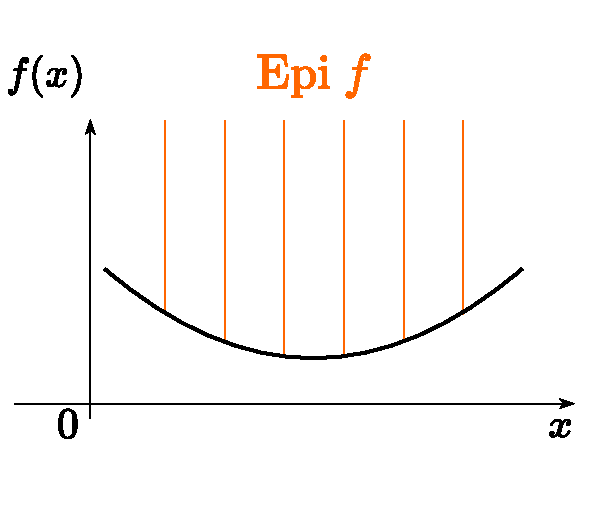
\includegraphics[keepaspectratio]{epigraph.pdf}}

}

\caption{Надграфик функции}

\end{figure}%

\subsection{Выпуклость надграфика = выпуклость
функции}\label{ux432ux44bux43fux443ux43aux43bux43eux441ux442ux44c-ux43dux430ux434ux433ux440ux430ux444ux438ux43aux430-ux432ux44bux43fux443ux43aux43bux43eux441ux442ux44c-ux444ux443ux43dux43aux446ux438ux438-1}

\begin{enumerate}
\def\labelenumi{\arabic{enumi}.}
\item
  \textbf{Необходимость}: Предположим, что \(f(x)\) выпукла на \(X\).
  Возьмем любые две произвольные точки \([x_1, \mu_1] \in \text{epi}f\)
  и \([x_2, \mu_2] \in \text{epi}f\). Также возьмем
  \(0 \leq \lambda \leq 1\) и обозначим
  \(x_{\lambda} = \lambda x_1 + (1 - \lambda) x_2, \mu_{\lambda} = \lambda \mu_1 + (1 - \lambda) \mu_2\).
  Тогда, \[
  \lambda\begin{bmatrix}x_1\\ \mu_1\end{bmatrix} + (1 - \lambda)\begin{bmatrix}x_2\\ \mu_2\end{bmatrix} = \begin{bmatrix}x_{\lambda}\\ \mu_{\lambda}\end{bmatrix}.
  \] Из выпуклости множества \(X\) следует, что \(x_{\lambda} \in X\).
  Кроме того, поскольку \(f(x)\) выпуклая функция, \[
  f(x_{\lambda}) \leq \lambda f(x_1) + (1 - \lambda) f(x_2) \leq \lambda \mu_1 + (1 - \lambda) \mu_2 = \mu_{\lambda}
  \] Неравенство выше означает, что
  \(\begin{bmatrix}x_{\lambda}\\ \mu_{\lambda}\end{bmatrix} \in \text{epi}f\).
  Таким образом, надграфик функции \(f\) является выпуклым множеством.
\item
  \textbf{Достаточность}: Предположим, что надграфик функции \(f\),
  \(\text{epi}f\), является выпуклым множеством. Тогда, из
  принадлежности точек \([x_1, \mu_1]\) и \([x_2, \mu_2]\) надграфику
  функции \(f\), следует, что

  \[
  \begin{bmatrix}x_{\lambda}\\ \mu_{\lambda}\end{bmatrix} =  \lambda\begin{bmatrix}x_1\\ \mu_1\end{bmatrix} + (1 - \lambda)\begin{bmatrix}x_2\\ \mu_2\end{bmatrix} \in \text{epi}f
  \] для любого \(0 \leq \lambda \leq 1\), т.е.
  \(f(x_{\lambda}) \leq \mu_{\lambda} = \lambda \mu_1 + (1 - \lambda) \mu_2\).
  Но это верно для всех \(\mu_1 \geq f(x_1)\) и \(\mu_2 \geq f(x_2)\), в
  частности, когда \(\mu_1 = f(x_1)\) и \(\mu_2 = f(x_2)\).
  Следовательно, мы приходим к неравенству \[
  f(x_{\lambda}) = f (\lambda x_1 + (1 - \lambda) x_2) \leq \lambda f(x_1) + (1 - \lambda) f(x_2).
  \]

  Поскольку точки \(x_1 \in X\) и \(x_2 \in X\) могут быть выбраны
  произвольно, \(f(x)\) является выпуклой функцией на \(X\).
\end{enumerate}

\subsection{Конус
нормы}\label{ux43aux43eux43dux443ux441-ux43dux43eux440ux43cux44b}

Пусть норма \(\Vert \cdot \Vert\) определена в пространстве \(U\).
Рассмотрим множество: \[
K := \{(x,t) \in U \times \mathbb{R}^+ : \Vert x \Vert \leq t \}
\] которое представляет собой надграфик функции
\(x \mapsto \Vert x \Vert\). Это множество называется конусом нормы.
Согласно утверждению выше, множество \(K\) является выпуклым.
\href{https://colab.research.google.com/github/MerkulovDaniil/optim/blob/master/assets/Notebooks/Norm_cones.ipynb}{\faPython Код
для рисунков}

\begin{figure}[H]

{\centering \pandocbounded{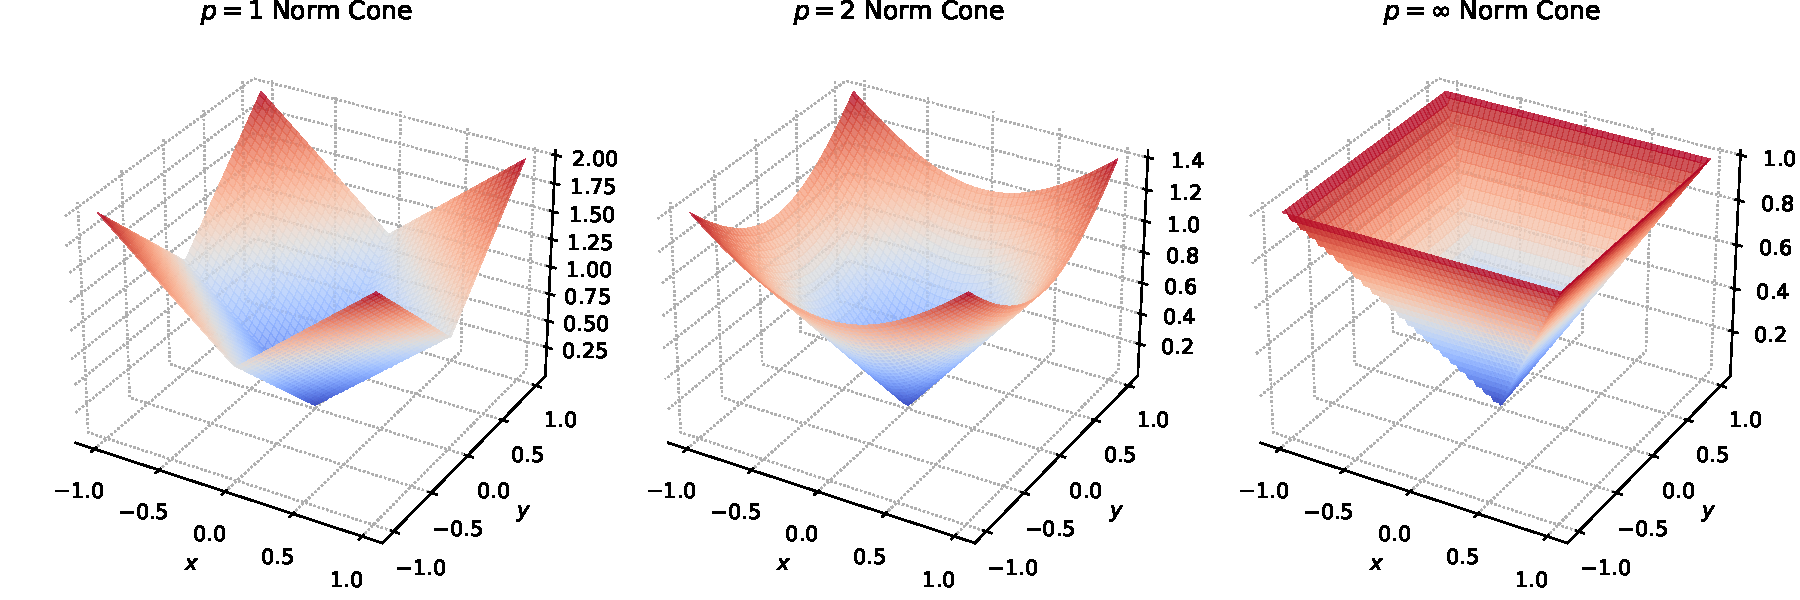
\includegraphics[keepaspectratio]{norm_cones.pdf}}

}

\caption{Конусы нормы для разных \(p\) - норм}

\end{figure}%

\subsection{Множество
подуровня}\label{ux43cux43dux43eux436ux435ux441ux442ux432ux43e-ux43fux43eux434ux443ux440ux43eux432ux43dux44f}

\begin{figure}[H]

{\centering \pandocbounded{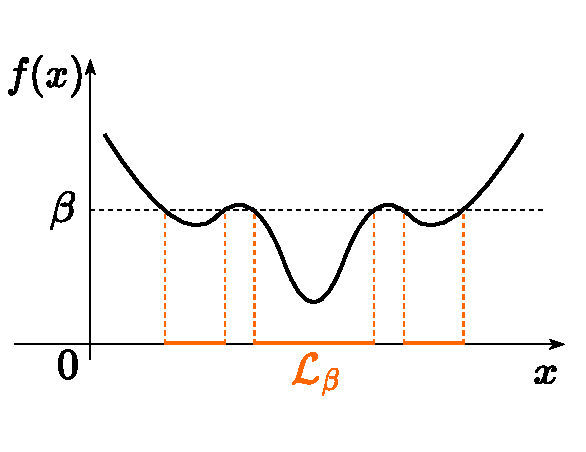
\includegraphics[keepaspectratio]{sublevel_set.pdf}}

}

\caption{Множество подуровня функции с уровнем \(\beta\)}

\end{figure}%

Для функции \(f(x)\), определенной на \(S \subseteq \mathbb{R}^n\),
следующее множество:

\[
\mathcal{L}_\beta = \left\{ x\in S : f(x) \le \beta\right\}
\]

называется \textbf{множеством подуровня} или множеством Лебега функции
\(f(x)\).

Обратите внимание, что если функция \(f(x)\) выпукла, то ее множества
подуровня выпуклы для любого \(\beta \in \mathbb{R}\).

Однако \textbf{обратное неверно}. (Рассмотрим функцию
\(f(x) = \sqrt{|x|}\))

\subsection{Сведение к
прямой}\label{ux441ux432ux435ux434ux435ux43dux438ux435-ux43a-ux43fux440ux44fux43cux43eux439}

\(f: S \to \mathbb{R}\) выпукла тогда и только тогда, когда \(S\)
выпукло и функция \(g(t) = f(x + tv)\) определена на
\(\left\{ t \mid x + tv \in S \right\}\) и выпукла для любого
\(x \in S, v \in \mathbb{R}^n\), что позволяет проверять выпуклость
скалярной функции для установления выпуклости векторной функции.

Если существует направление \(v\) для которого \(g(t)\) не выпукло, то
\(f\) не выпукла. \begin{center}
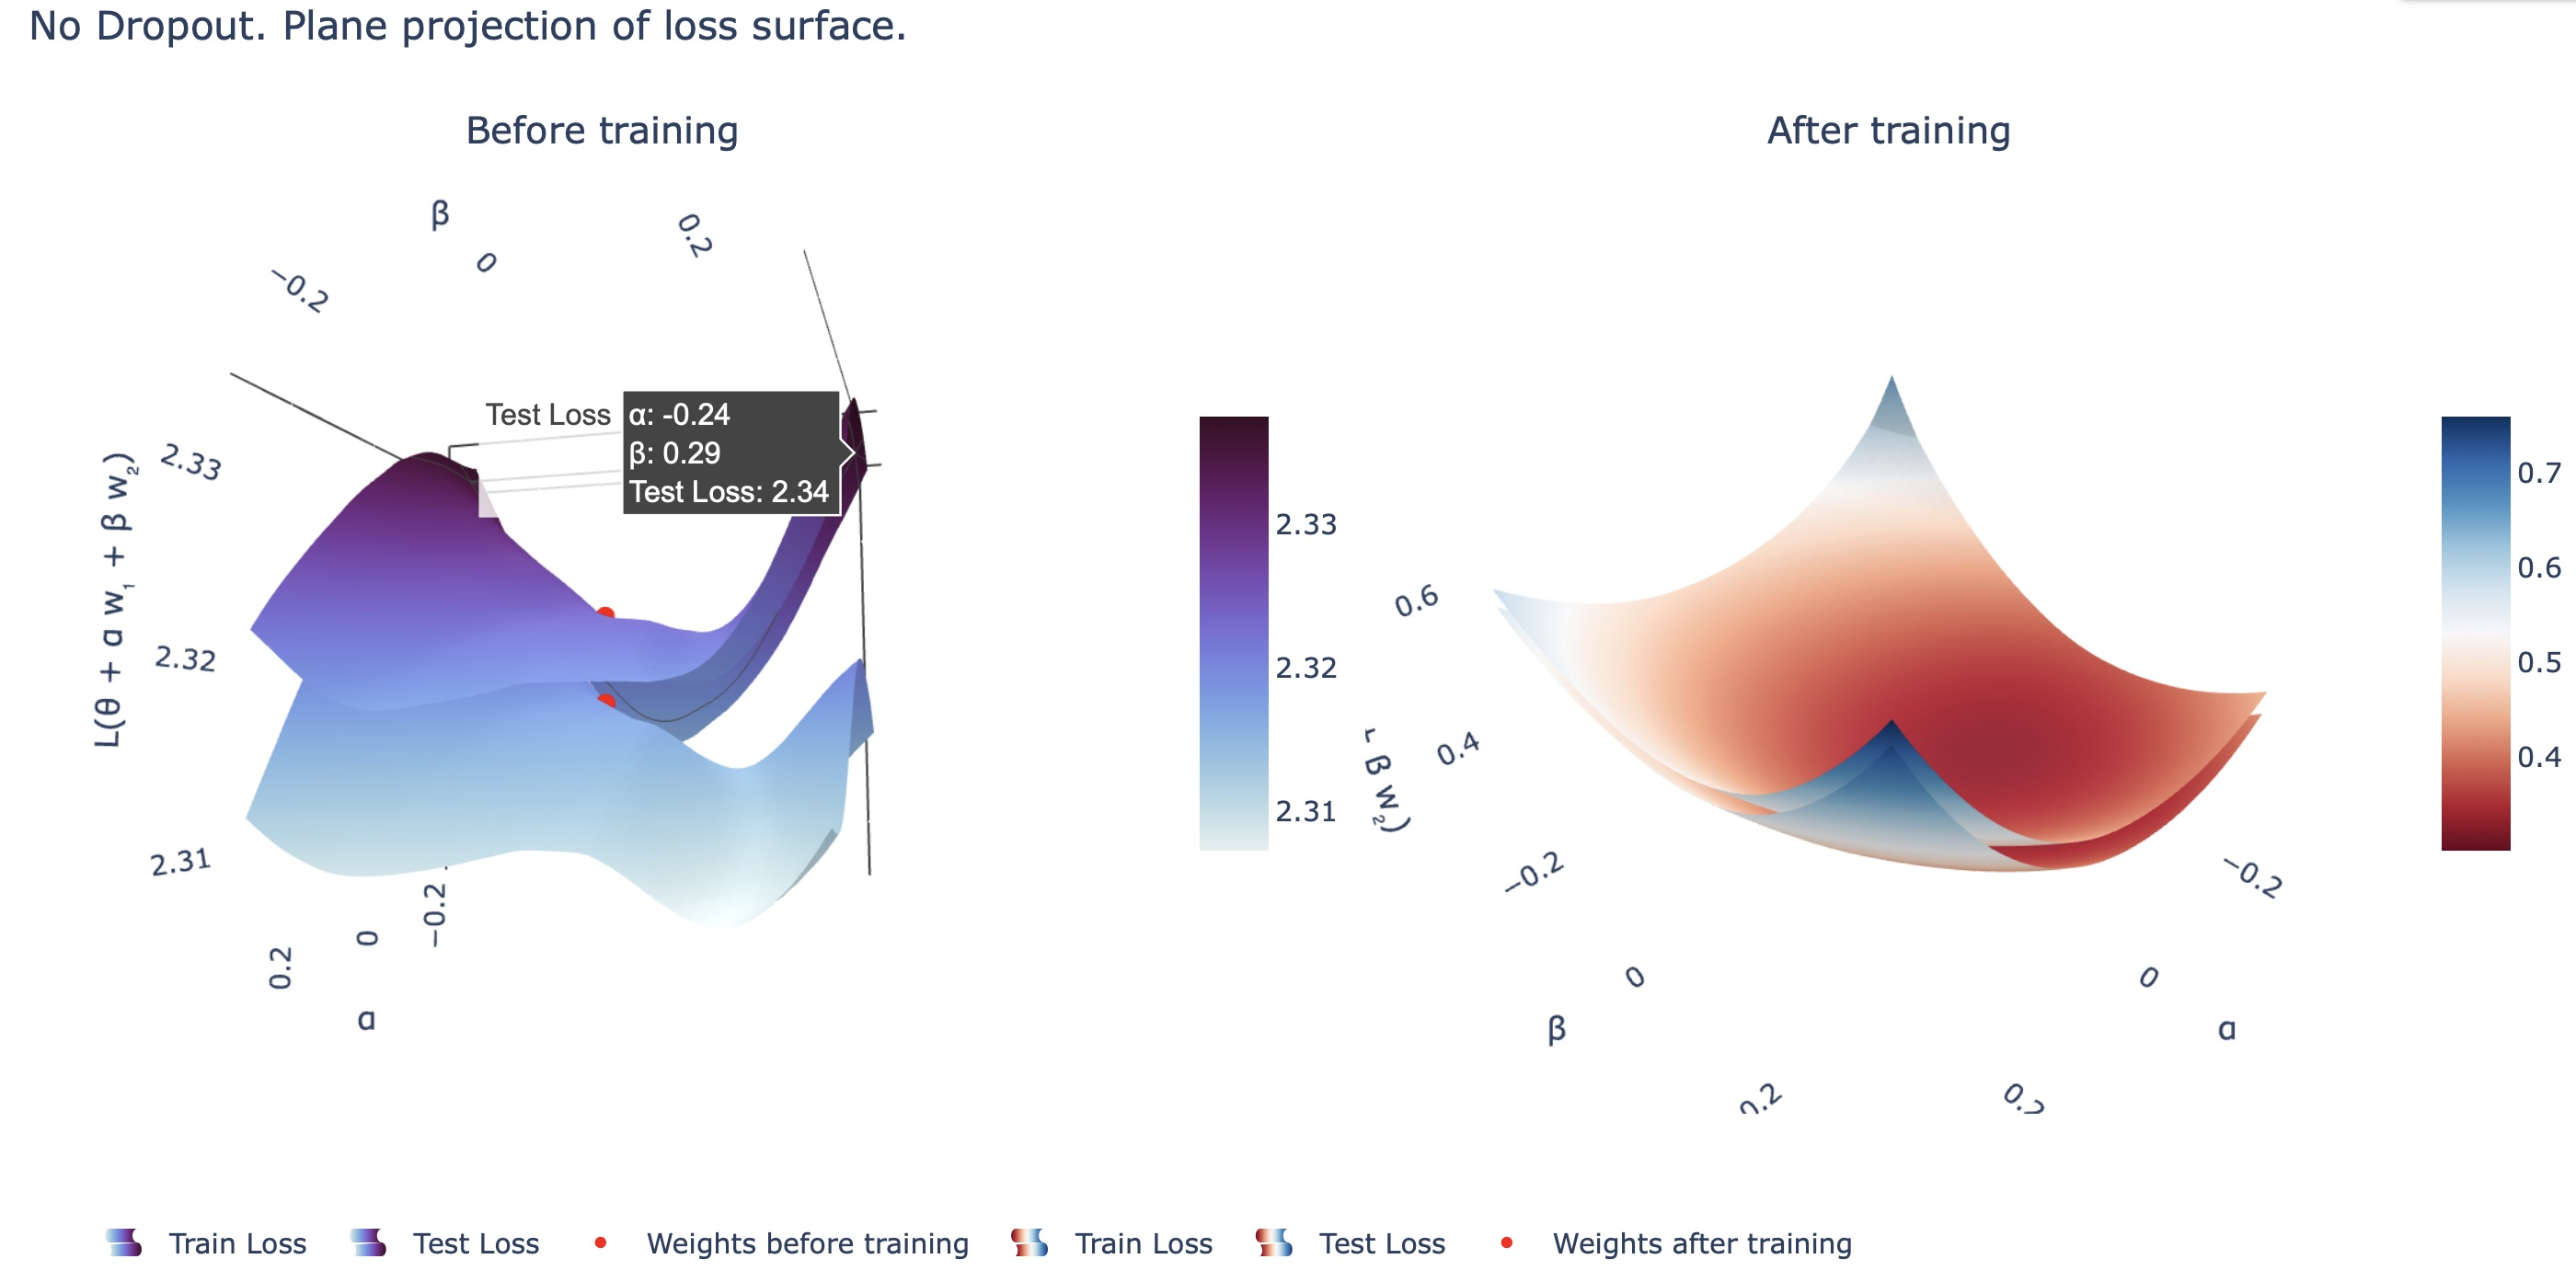
\includegraphics[width=0.8\linewidth,height=\textheight,keepaspectratio]{plane_projection.jpeg}
\end{center}

\subsection{Операции, сохраняющие
выпуклость}\label{ux43eux43fux435ux440ux430ux446ux438ux438-ux441ux43eux445ux440ux430ux43dux44fux44eux449ux438ux435-ux432ux44bux43fux443ux43aux43bux43eux441ux442ux44c-1}

\begin{figure}[H]

{\centering 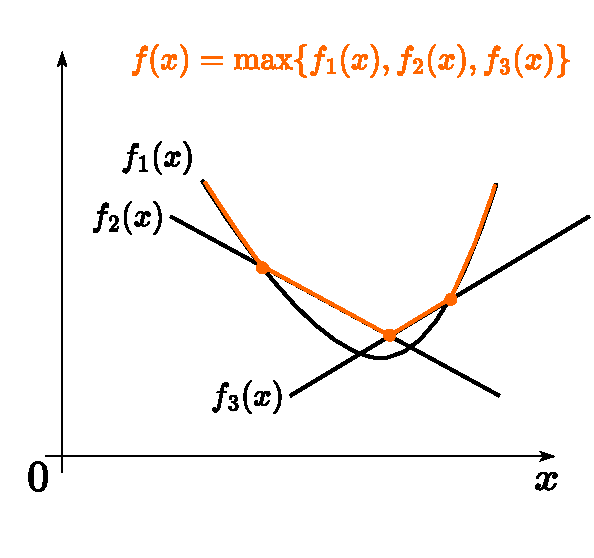
\includegraphics[width=0.7\linewidth,height=\textheight,keepaspectratio]{pointwise_maximum.pdf}

}

\caption{Поточечный максимум (супремум) выпуклых функций выпуклый}

\end{figure}%

\begin{itemize}
\tightlist
\item
  Поточечный максимум (супремум) любого числа функций: Если
  \(f_1(x), \ldots, f_m(x)\) выпуклы, то
  \(f(x) = \max \{f_1(x), \ldots, f_m(x)\}\) выпукла.
\item
  Неотрицательная сумма выпуклых функций:
  \(\alpha f(x) + \beta g(x), (\alpha \geq 0 , \beta \geq 0)\).
\item
  Композиция с аффинной функцией \(f(Ax + b)\) выпукла, если \(f(x)\)
  выпукла.
\item
  Если \(f(x,y)\) выпукла по \(x\) для любого \(y \in Y\):
  \(g(x) = \underset{y \in Y}{\text{sup}}f(x,y)\) также выпукла.
\item
  Если \(f(x)\) выпукла на \(S\), то \(g(x,t) = t f(x/t)\) - выпукла с
  \(x/t \in S, t > 0\).
\item
  Пусть \(f_1: S_1 \to \mathbb{R}\) и \(f_2: S_2 \to \mathbb{R}\), где
  \(\text{range}(f_1) \subseteq S_2\). Если \(f_1\) и \(f_2\) выпуклы, и
  \(f_2\) возрастает, то \(f_2 \circ f_1\) выпукла на \(S_1\).
\end{itemize}

\subsection{Функция максимального собственного значения матрицы является
выпуклой}\label{ux444ux443ux43dux43aux446ux438ux44f-ux43cux430ux43aux441ux438ux43cux430ux43bux44cux43dux43eux433ux43e-ux441ux43eux431ux441ux442ux432ux435ux43dux43dux43eux433ux43e-ux437ux43dux430ux447ux435ux43dux438ux44f-ux43cux430ux442ux440ux438ux446ux44b-ux44fux432ux43bux44fux435ux442ux441ux44f-ux432ux44bux43fux443ux43aux43bux43eux439}

\begin{tcolorbox}[enhanced jigsaw, colframe=quarto-callout-color-frame, titlerule=0mm, coltitle=black, toprule=.15mm, colback=white, leftrule=.75mm, bottomtitle=1mm, toptitle=1mm, colbacktitle=quarto-callout-color!10!white, breakable, opacityback=0, bottomrule=.15mm, left=2mm, opacitybacktitle=0.6, title=\textcolor{quarto-callout-color}{\faInfo}\hspace{0.5em}{Example}, rightrule=.15mm, arc=.35mm]

Покажите, что \(f(A) = \lambda_{max}(A)\) - выпукла, если \(A \in S^n\).

\end{tcolorbox}

\section{Критерии сильной
выпуклости}\label{ux43aux440ux438ux442ux435ux440ux438ux438-ux441ux438ux43bux44cux43dux43eux439-ux432ux44bux43fux443ux43aux43bux43eux441ux442ux438}

\subsection{Дифференциальный критерий выпуклости первого
порядка}\label{ux434ux438ux444ux444ux435ux440ux435ux43dux446ux438ux430ux43bux44cux43dux44bux439-ux43aux440ux438ux442ux435ux440ux438ux439-ux432ux44bux43fux443ux43aux43bux43eux441ux442ux438-ux43fux435ux440ux432ux43eux433ux43e-ux43fux43eux440ux44fux434ux43aux430}

Дифференцируемая функция \(f(x)\) определенная на выпуклом множестве
\(S \subseteq \mathbb{R}^n\) выпукла тогда и только тогда, когда
\(\forall x,y \in S\): \[
f(y) \ge f(x) + \nabla f^T(x)(y-x)
\] Пусть \(y = x + \Delta x\), тогда критерий запишется в виде: \[
f(x + \Delta x) \ge f(x) + \nabla f^T(x)\Delta x
\]

\begin{figure}[H]

{\centering \pandocbounded{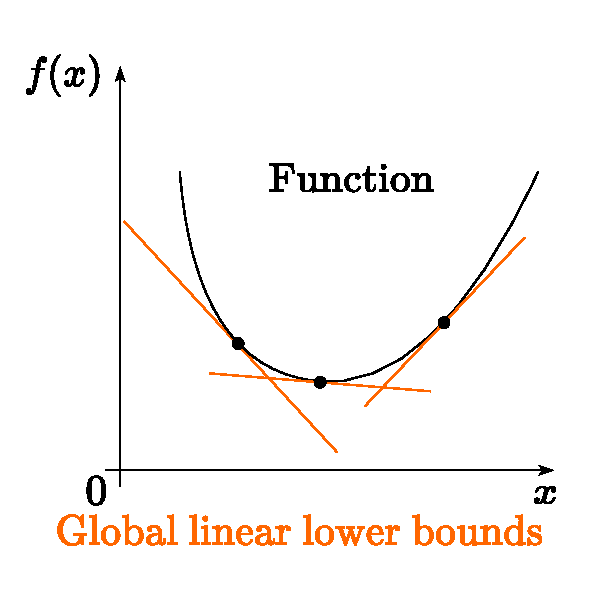
\includegraphics[keepaspectratio]{global_linear_lower_bound.pdf}}

}

\caption{Выпуклая функция больше или равна линейной аппроксимации
Тейлора в любой точке}

\end{figure}%

\subsection{Дифференциальный критерий выпуклости второго
порядка}\label{ux434ux438ux444ux444ux435ux440ux435ux43dux446ux438ux430ux43bux44cux43dux44bux439-ux43aux440ux438ux442ux435ux440ux438ux439-ux432ux44bux43fux443ux43aux43bux43eux441ux442ux438-ux432ux442ux43eux440ux43eux433ux43e-ux43fux43eux440ux44fux434ux43aux430}

Дважды дифференцируемая функция \(f(x)\) определенная на выпуклом
множестве \(S \subseteq \mathbb{R}^n\) выпукла тогда и только тогда,
когда \(\forall x \in \mathbf{int}(S) \neq \emptyset\): \[
\nabla^2 f(x) \succeq 0
\] Другими словами, \(\forall y \in \mathbb{R}^n\): \[
\langle y, \nabla^2f(x)y\rangle \geq 0
\]

\subsection{Сильная
выпуклость}\label{ux441ux438ux43bux44cux43dux430ux44f-ux432ux44bux43fux443ux43aux43bux43eux441ux442ux44c}

\(f(x)\), \textbf{определенная на выпуклом множестве}
\(S \subseteq \mathbb{R}^n\), называется \(\mu\)-сильно выпуклой (сильно
выпуклой) на \(S\), если: \[
f(\lambda x_1 + (1 - \lambda)x_2) \le \lambda f(x_1) + (1 - \lambda)f(x_2) - \frac{\mu}{2} \lambda (1 - \lambda)\|x_1 - x_2\|^2
\] для любых \(x_1, x_2 \in S\) и \(0 \le \lambda \le 1\) для некоторого
\(\mu > 0\).

\begin{figure}[H]

{\centering \pandocbounded{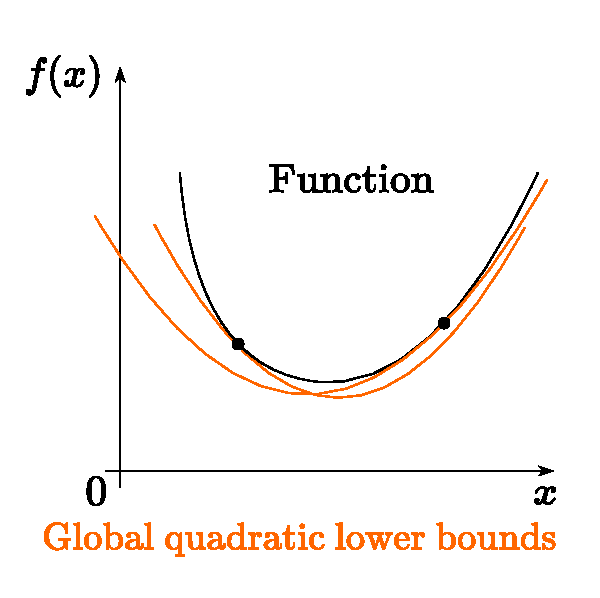
\includegraphics[keepaspectratio]{global_quad_lower_bound.pdf}}

}

\caption{Сильно выпуклая функция не меньше некоторой параболы в любой
точке}

\end{figure}%

\subsection{Дифференциальный критерий сильной выпуклости первого
порядка}\label{ux434ux438ux444ux444ux435ux440ux435ux43dux446ux438ux430ux43bux44cux43dux44bux439-ux43aux440ux438ux442ux435ux440ux438ux439-ux441ux438ux43bux44cux43dux43eux439-ux432ux44bux43fux443ux43aux43bux43eux441ux442ux438-ux43fux435ux440ux432ux43eux433ux43e-ux43fux43eux440ux44fux434ux43aux430}

Дифференцируемая \(f(x)\) определенная на выпуклом множестве
\(S \subseteq \mathbb{R}^n\) является \(\mu\)-сильно выпуклой тогда и
только тогда, когда \(\forall x,y \in S\): \[
f(y) \ge f(x) + \nabla f^T(x)(y-x) + \dfrac{\mu}{2}\|y-x\|^2
\]

Пусть \(y = x + \Delta x\), тогда критерий запишется в виде: \[
f(x + \Delta x) \ge f(x) + \nabla f^T(x)\Delta x + \dfrac{\mu}{2}\|\Delta x\|^2
\]

\begin{tcolorbox}[enhanced jigsaw, colframe=quarto-callout-color-frame, titlerule=0mm, coltitle=black, toprule=.15mm, colback=white, leftrule=.75mm, bottomtitle=1mm, toptitle=1mm, colbacktitle=quarto-callout-color!10!white, breakable, opacityback=0, bottomrule=.15mm, left=2mm, opacitybacktitle=0.6, title=\textcolor{quarto-callout-color}{\faInfo}\hspace{0.5em}{Theorem}, rightrule=.15mm, arc=.35mm]

Пусть \(f(x)\) дифференцируемая функция на выпуклом множестве
\(X \subseteq \mathbb{R}^n\). Тогда \(f(x)\) сильно выпукла на \(X\) с
константой \(\mu > 0\) тогда и только тогда, когда \[ 
f(x) - f(x_0) \geq \langle \nabla f(x_0), x - x_0 \rangle + \frac{\mu}{2} \| x - x_0 \|^2
\] для всех \(x, x_0 \in X\).

\end{tcolorbox}

\textbf{Доказательство.} \emph{Необходимость}

Пусть \(0 < \lambda \leq 1\). Согласно определению сильно выпуклой
функции, \[ 
f(\lambda x + (1 - \lambda) x_0) \leq \lambda f(x) + (1 - \lambda) f(x_0) - \frac{\mu}{2} \lambda (1 - \lambda) \| x - x_0 \|^2 
\]

или эквивалентно, \[ 
f(x) - f(x_0) - \frac{\mu}{2} (1 - \lambda) \| x - x_0 \|^2 \geq \frac{1}{\lambda} [f(\lambda x + (1 - \lambda) x_0) - f(x_0)] = 
\]

\[ 
= \frac{1}{\lambda} [f(x_0 + \lambda(x - x_0)) - f(x_0)] = \frac{1}{\lambda} [\lambda \langle \nabla f(x_0), x - x_0 \rangle + o(\lambda)] = 
\]

\[
= \langle \nabla f(x_0), x - x_0 \rangle + \frac{o(\lambda)}{\lambda}. 
\] Таким образом, переходя к пределу при \(\lambda \downarrow 0\), мы
приходим к исходному утверждению.

\emph{Достаточность}

Предположим, что неравенство в теореме выполняется для всех
\(x, x_0 \in X\). Возьмем \(x_0 = \lambda x_1 + (1 - \lambda) x_2\), где
\(x_1, x_2 \in X\), \(0 \leq \lambda \leq 1\). Согласно неравенству,
следующие неравенства выполняются:

\[ 
f(x_1) - f(x_0) \geq \langle \nabla f(x_0), x_1 - x_0 \rangle + \frac{\mu}{2} \| x_1 - x_0 \|^2, 
\] \[ 
f(x_2) - f(x_0) \geq \langle \nabla f(x_0), x_2 - x_0 \rangle + \frac{\mu}{2} \| x_2 - x_0 \|^2. 
\]

Умножая первое неравенство на \(\lambda\) и второе на \(1 - \lambda\) и
складывая их, учитывая, что \[ 
x_1 - x_0 = (1 - \lambda)(x_1 - x_2), \quad x_2 - x_0 = \lambda(x_2 - x_1), 
\]

и
\(\lambda(1 - \lambda)^2 + \lambda^2(1 - \lambda) = \lambda(1 - \lambda)\),
мы получаем \[ 
\begin{split}
\lambda f(x_1) + (1 - \lambda) f(x_2) - f(x_0) - \frac{\mu}{2} \lambda (1 - \lambda) \| x_1 - x_2 \|^2 \geq \\
\langle \nabla f(x_0), \lambda x_1 + (1 - \lambda) x_2 - x_0 \rangle = 0. 
\end{split}
\] Таким образом, неравенство из определения сильно выпуклой функции
выполняется. Важно отметить, что \(\mu = 0\) соответствует случаю
выпуклой функции и соответствующему дифференциальному критерию.

\subsection{Дифференциальный критерий сильной выпуклости второго
порядка}\label{ux434ux438ux444ux444ux435ux440ux435ux43dux446ux438ux430ux43bux44cux43dux44bux439-ux43aux440ux438ux442ux435ux440ux438ux439-ux441ux438ux43bux44cux43dux43eux439-ux432ux44bux43fux443ux43aux43bux43eux441ux442ux438-ux432ux442ux43eux440ux43eux433ux43e-ux43fux43eux440ux44fux434ux43aux430}

Дважды дифференцируемая функция \(f(x)\) определенная на выпуклом
множестве \(S \subseteq \mathbb{R}^n\) называется \(\mu\)-сильно
выпуклой тогда и только тогда, когда
\(\forall x \in \mathbf{int}(S) \neq \emptyset\): \[
\nabla^2 f(x) \succeq \mu I
\] Другими словами: \[
\langle y, \nabla^2f(x)y\rangle \geq \mu \|y\|^2
\]

\begin{tcolorbox}[enhanced jigsaw, colframe=quarto-callout-color-frame, titlerule=0mm, coltitle=black, toprule=.15mm, colback=white, leftrule=.75mm, bottomtitle=1mm, toptitle=1mm, colbacktitle=quarto-callout-color!10!white, breakable, opacityback=0, bottomrule=.15mm, left=2mm, opacitybacktitle=0.6, title=\textcolor{quarto-callout-color}{\faInfo}\hspace{0.5em}{Theorem}, rightrule=.15mm, arc=.35mm]

Пусть \(X \subseteq \mathbb{R}^n\) выпуклое множество, с
\(\text{int}X \neq \emptyset\). Кроме того, пусть \(f(x)\) дважды
непрерывно дифференцируемая функция на \(X\). Тогда \(f(x)\) сильно
выпукла на \(X\) с константой \(\mu > 0\) тогда и только тогда, когда \[
\langle y, \nabla^2 f(x) y \rangle \geq \mu \| y \|^2 \quad 
\] для всех \(x \in X\) и \(y \in \mathbb{R}^n\).

\end{tcolorbox}

\textbf{Доказательство.} \emph{Необходимость}

Целевое неравенство тривиально, когда \(y = \mathbf{0}_n\), поэтому мы
предполагаем \(y \neq \mathbf{0}_n\).

Предположим, что \(x\) является внутренней точкой множества \(X\). Тогда
\(x + \alpha y \in X\) для всех \(y \in \mathbb{R}^n\) и достаточно
малых \(\alpha\). Поскольку \(f(x)\) дважды дифференцируема, \[
f(x + \alpha y) = f(x) + \alpha \langle \nabla f(x), y \rangle + \frac{\alpha^2}{2} \langle y, \nabla^2 f(x) y \rangle + o(\alpha^2).
\]

На основании первого дифференциального критерия сильной выпуклости: \[
\frac{\alpha^2}{2} \langle y, \nabla^2 f(x) y \rangle + o(\alpha^2) = f(x + \alpha y) - f(x) - \alpha \langle \nabla f(x), y \rangle \geq \frac{\mu}{2} \alpha^2 \| y \|^2.
\]

Это неравенство сводится к целевому неравенству после деления обеих
сторон на \(\alpha^2\) и перехода к пределу при \(\alpha \downarrow 0\).

Если \(x \in X\) но \(x \notin \text{int}X\), рассмотрим
последовательность \(\{x_k\}\) такую, что \(x_k \in \text{int}X\) и
\(x_k \rightarrow x\) при \(k \rightarrow \infty\). Тогда, мы приходим к
целевому неравенству после перехода к пределу.

\emph{Достаточность}

Используя формулу Тейлора с остаточным членом Лагранжа и целевое
неравенство, мы получаем для \(x + y \in X\): \[
f(x + y) - f(x) - \langle \nabla f(x), y \rangle = \frac{1}{2} \langle y, \nabla^2 f(x + \alpha y) y \rangle \geq \frac{\mu}{2} \| y \|^2, 
\] где \(0 \leq \alpha \leq 1\). Следовательно,

\[
f(x + y) - f(x) \geq \langle \nabla f(x), y \rangle + \frac{\mu}{2} \| y \|^2.
\] Следовательно, согласно первому дифференциальному критерию сильной
выпуклости, функция \(f(x)\) сильно выпукла с константой \(\mu\). Важно
отметить, что \(\mu = 0\) соответствует случаю выпуклой функции и
соответствующему дифференциальному критерию.

\subsection{Выпуклая и вогнутая
функция}\label{ux432ux44bux43fux443ux43aux43bux430ux44f-ux438-ux432ux43eux433ux43dux443ux442ux430ux44f-ux444ux443ux43dux43aux446ux438ux44f}

\begin{tcolorbox}[enhanced jigsaw, colframe=quarto-callout-color-frame, titlerule=0mm, coltitle=black, toprule=.15mm, colback=white, leftrule=.75mm, bottomtitle=1mm, toptitle=1mm, colbacktitle=quarto-callout-color!10!white, breakable, opacityback=0, bottomrule=.15mm, left=2mm, opacitybacktitle=0.6, title=\textcolor{quarto-callout-color}{\faInfo}\hspace{0.5em}{Example}, rightrule=.15mm, arc=.35mm]

Покажите, что \(f(x) = c^\top x + b\) выпукла и вогнута.

\end{tcolorbox}

\subsection{Простейшая сильно выпуклая
функция}\label{ux43fux440ux43eux441ux442ux435ux439ux448ux430ux44f-ux441ux438ux43bux44cux43dux43e-ux432ux44bux43fux443ux43aux43bux430ux44f-ux444ux443ux43dux43aux446ux438ux44f}

\begin{tcolorbox}[enhanced jigsaw, colframe=quarto-callout-color-frame, titlerule=0mm, coltitle=black, toprule=.15mm, colback=white, leftrule=.75mm, bottomtitle=1mm, toptitle=1mm, colbacktitle=quarto-callout-color!10!white, breakable, opacityback=0, bottomrule=.15mm, left=2mm, opacitybacktitle=0.6, title=\textcolor{quarto-callout-color}{\faInfo}\hspace{0.5em}{Example}, rightrule=.15mm, arc=.35mm]

Покажите, что \(f(x) = x^\top Ax\), где \(A\succeq 0\) - выпукла на
\(\mathbb{R}^n\). Является ли она сильно выпуклой?

\end{tcolorbox}

\subsection{Выпуклость и
непрерывность}\label{ux432ux44bux43fux443ux43aux43bux43eux441ux442ux44c-ux438-ux43dux435ux43fux440ux435ux440ux44bux432ux43dux43eux441ux442ux44c}

Пусть \(f(x)\) - выпуклая функция на выпуклом множестве
\(S \subseteq \mathbb{R}^n\). Тогда \(f(x)\) непрерывна
\(\forall x \in \textbf{ri}(S)\).

\begin{tcolorbox}[enhanced jigsaw, colframe=quarto-callout-color-frame, titlerule=0mm, coltitle=black, toprule=.15mm, colback=white, leftrule=.75mm, bottomtitle=1mm, toptitle=1mm, colbacktitle=quarto-callout-color!10!white, breakable, opacityback=0, bottomrule=.15mm, left=2mm, opacitybacktitle=0.6, title=\textcolor{quarto-callout-color}{\faInfo}\hspace{0.5em}{Собственная выпуклая функция}, rightrule=.15mm, arc=.35mm]

Функция \(f: \mathbb{R}^n \rightarrow \mathbb{R}\) называется
\textbf{собственной выпуклой функцией}, если она никогда не принимает
значения \(-\infty\) и не равна \(\infty\) тождественно.

\end{tcolorbox}

\begin{tcolorbox}[enhanced jigsaw, colframe=quarto-callout-color-frame, titlerule=0mm, coltitle=black, toprule=.15mm, colback=white, leftrule=.75mm, bottomtitle=1mm, toptitle=1mm, colbacktitle=quarto-callout-color!10!white, breakable, opacityback=0, bottomrule=.15mm, left=2mm, opacitybacktitle=0.6, title=\textcolor{quarto-callout-color}{\faInfo}\hspace{0.5em}{Индикаторная функция}, rightrule=.15mm, arc=.35mm]

\[
\delta_S(x) = \begin{cases} \infty, &x \in S, \\ 0, &x \notin S, \end{cases}
\] является собственной выпуклой функцией.

\end{tcolorbox}

\begin{tcolorbox}[enhanced jigsaw, colframe=quarto-callout-color-frame, titlerule=0mm, coltitle=black, toprule=.15mm, colback=white, leftrule=.75mm, bottomtitle=1mm, toptitle=1mm, colbacktitle=quarto-callout-color!10!white, breakable, opacityback=0, bottomrule=.15mm, left=2mm, opacitybacktitle=0.6, title=\textcolor{quarto-callout-color}{\faInfo}\hspace{0.5em}{Замкнутая функция}, rightrule=.15mm, arc=.35mm]

Функция \(f: \mathbb{R}^n \rightarrow \mathbb{R}\) называется
\textbf{замкнутой}, если для каждого \(\alpha \in \mathbb{R}\),
множество подуровня замкнуто.

Эквивалентно, если надграфик замкнут, то функция \(f\) замкнута.

\end{tcolorbox}

\begin{figure}[H]

{\centering 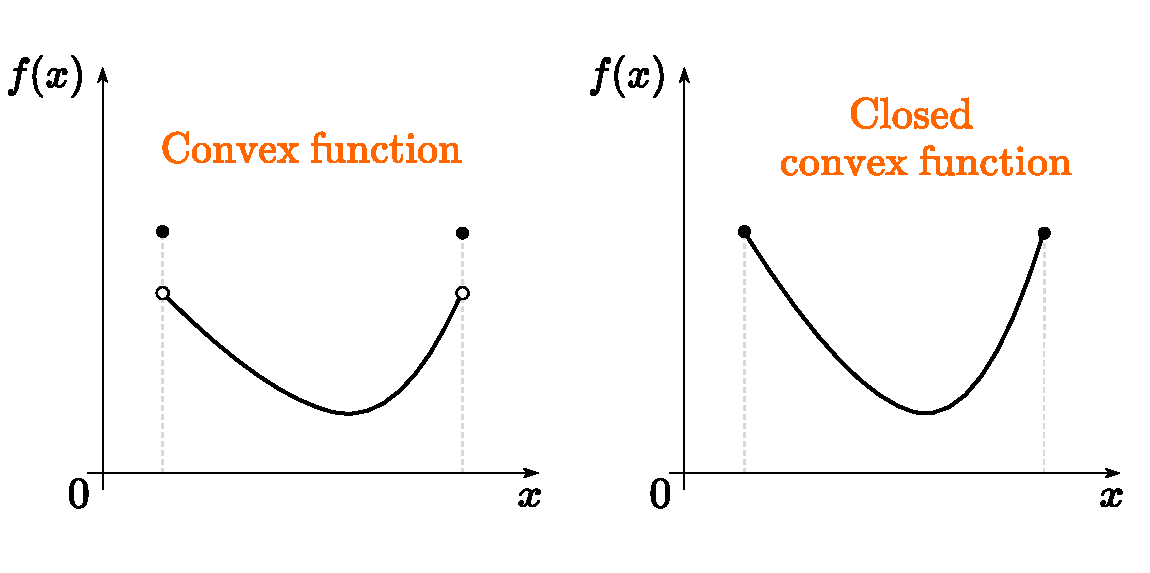
\includegraphics[width=0.88\linewidth,height=\textheight,keepaspectratio]{closed_function.pdf}

}

\caption{Выпуклые функции могут иметь разрывы на границе своей области
определения.}

\end{figure}%

\subsection{Факты о
выпуклости}\label{ux444ux430ux43aux442ux44b-ux43e-ux432ux44bux43fux443ux43aux43bux43eux441ux442ux438}

\begin{itemize}
\item
  \(f(x)\) называется (строго, сильно) вогнутой, если функция \(-f(x)\)
  - (строго, сильно) выпукла.
\item
  Неравенство Йенсена для выпуклых функций: \[
   f \left( \sum\limits_{i=1}^n \alpha_i x_i \right) \leq \sum\limits_{i=1}^n \alpha_i f(x_i)
   \] для \(\alpha_i \geq 0; \quad \sum\limits_{i=1}^n \alpha_i = 1\)
  (вероятностный симплекс)

  Для непрерывного случая:\\
  \[
   f \left( \int\limits_{S} x p(x)dx \right) \leq \int\limits_{S} f(x)p(x)dx
   \] Если интегралы существуют и
  \(p(x) \geq 0, \quad \int\limits_{S} p(x)dx = 1\).
\item
  Если функция \(f(x)\) и множество \(S\) выпуклы, то любой локальный
  минимум \(x^* = \text{arg}\min\limits_{x \in S} f(x)\) будет
  глобальным. Сильная выпуклость гарантирует единственность решения.
\end{itemize}

\subsection{Другие формы
выпуклости}\label{ux434ux440ux443ux433ux438ux435-ux444ux43eux440ux43cux44b-ux432ux44bux43fux443ux43aux43bux43eux441ux442ux438}

\begin{itemize}
\tightlist
\item
  Логарифмическая выпуклость: \(\log f\) выпукла; Логарифмическая
  выпуклость влечет выпуклость.
\item
  Логарифмическая вогнутость: \(\log f\) вогнута; \textbf{не} замкнута
  относительно сложения!
\item
  Экспоненциальная выпуклость: \([f(x_i + x_j)] \succeq 0\), для
  \(x_1, \ldots, x_n\)
\item
  Операторная выпуклость: \(f(\lambda X + (1 - \lambda )Y)\)
\item
  Квазивыпуклость:
  \(f(\lambda x + (1 - \lambda) y) \leq \max \{f(x), f(y)\}\)
\item
  Псевдовыпуклость:
  \(\langle \nabla f(y), x - y \rangle \geq 0 \longrightarrow f(x) \geq f(y)\)
\item
  Дискретная выпуклость: \(f : \mathbb{Z}^n \to \mathbb{Z}\);
  ``выпуклость + теория матроидов.''
\end{itemize}

\subsection{Условие Поляка-Лоясиевича. Линейная сходимость градиентного
спуска без
выпуклости}\label{ux443ux441ux43bux43eux432ux438ux435-ux43fux43eux43bux44fux43aux430-ux43bux43eux44fux441ux438ux435ux432ux438ux447ux430.-ux43bux438ux43dux435ux439ux43dux430ux44f-ux441ux445ux43eux434ux438ux43cux43eux441ux442ux44c-ux433ux440ux430ux434ux438ux435ux43dux442ux43dux43eux433ux43e-ux441ux43fux443ux441ux43aux430-ux431ux435ux437-ux432ux44bux43fux443ux43aux43bux43eux441ux442ux438}

Неравенство PL выполняется, если выполняется следующее условие для
некоторого \(\mu > 0\), \[
\Vert \nabla f(x) \Vert^2 \geq 2\mu (f(x) - f^*) \forall x
\] При выполнении условия PL алгоритм градиентного спуска имеет линейную
сходимость.

Следующие функции удовлетворяют условию PL, но не являются выпуклыми.
\href{https://colab.research.google.com/github/MerkulovDaniil/optim/blob/master/assets/Notebooks/PL_function.ipynb}{\faPython Ссылка
на код}

\[
f(x) = x^2 + 3\sin^2(x)
\]

\begin{figure}[H]

{\centering 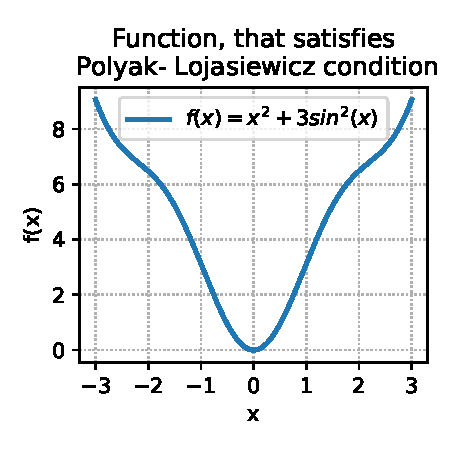
\includegraphics[width=0.45\linewidth,height=\textheight,keepaspectratio]{pl_2d.pdf}

}

\caption{Функция PL}

\end{figure}%

\[
f(x,y) = \dfrac{(y - \sin x)^2}{2}
\]

\begin{figure}[H]

{\centering 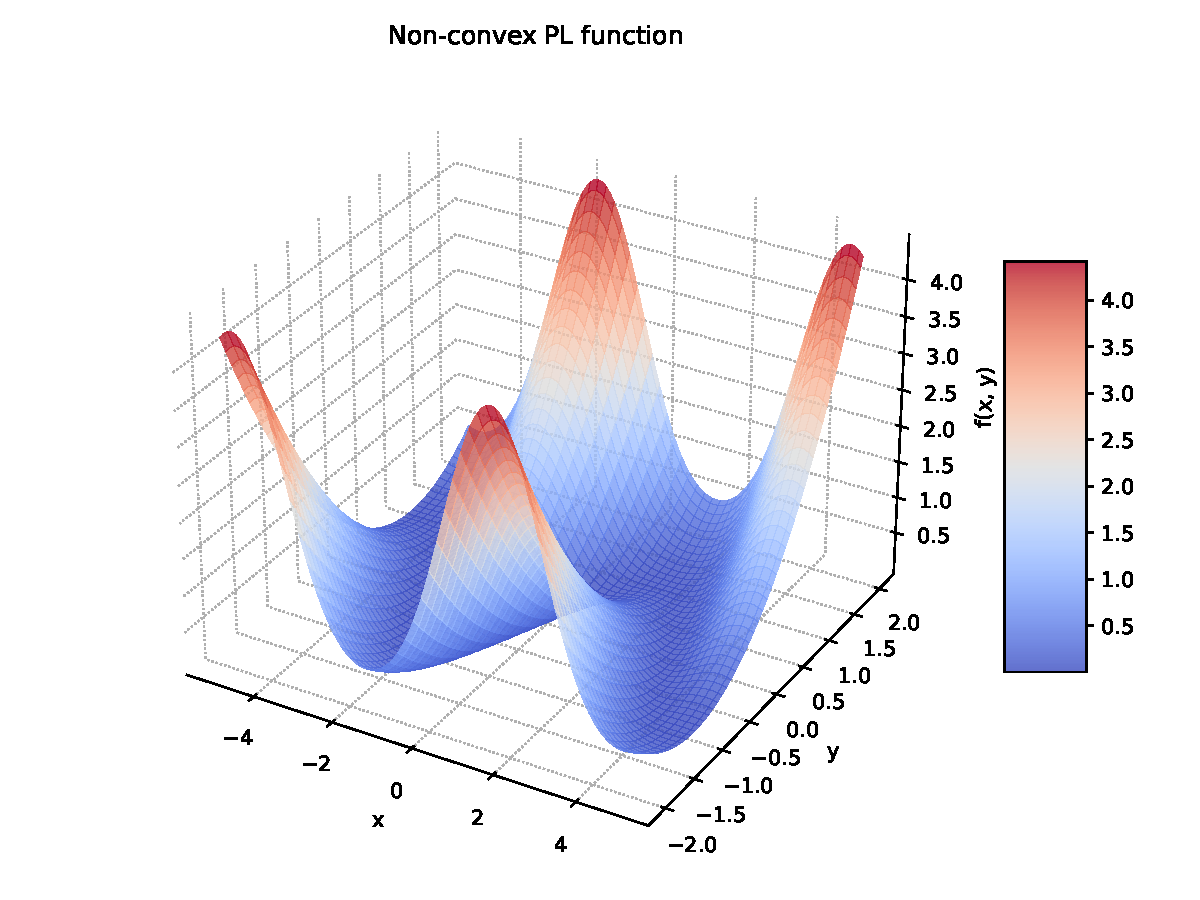
\includegraphics[width=0.8\linewidth,height=\textheight,keepaspectratio]{pl_3d.pdf}

}

\caption{Функция PL}

\end{figure}%

\section{Выпуклость в машинном
обучении}\label{ux432ux44bux43fux443ux43aux43bux43eux441ux442ux44c-ux432-ux43cux430ux448ux438ux43dux43dux43eux43c-ux43eux431ux443ux447ux435ux43dux438ux438}

\subsection[Метод наименьших квадратов aka линейная регрессия
]{\texorpdfstring{Метод наименьших квадратов aka линейная регрессия
\footnote{Посмотрите на
  \href{https://colab.research.google.com/github/MerkulovDaniil/optim/blob/master/assets/Notebooks/Real_world_LLS_exercise.ipynb}{\faPython пример}
  реальных данных линейной задачи метода наименьших квадратов}}{Метод наименьших квадратов aka линейная регрессия }}\label{ux43cux435ux442ux43eux434-ux43dux430ux438ux43cux435ux43dux44cux448ux438ux445-ux43aux432ux430ux434ux440ux430ux442ux43eux432-aka-ux43bux438ux43dux435ux439ux43dux430ux44f-ux440ux435ux433ux440ux435ux441ux441ux438ux44f}

\begin{figure}[H]

{\centering 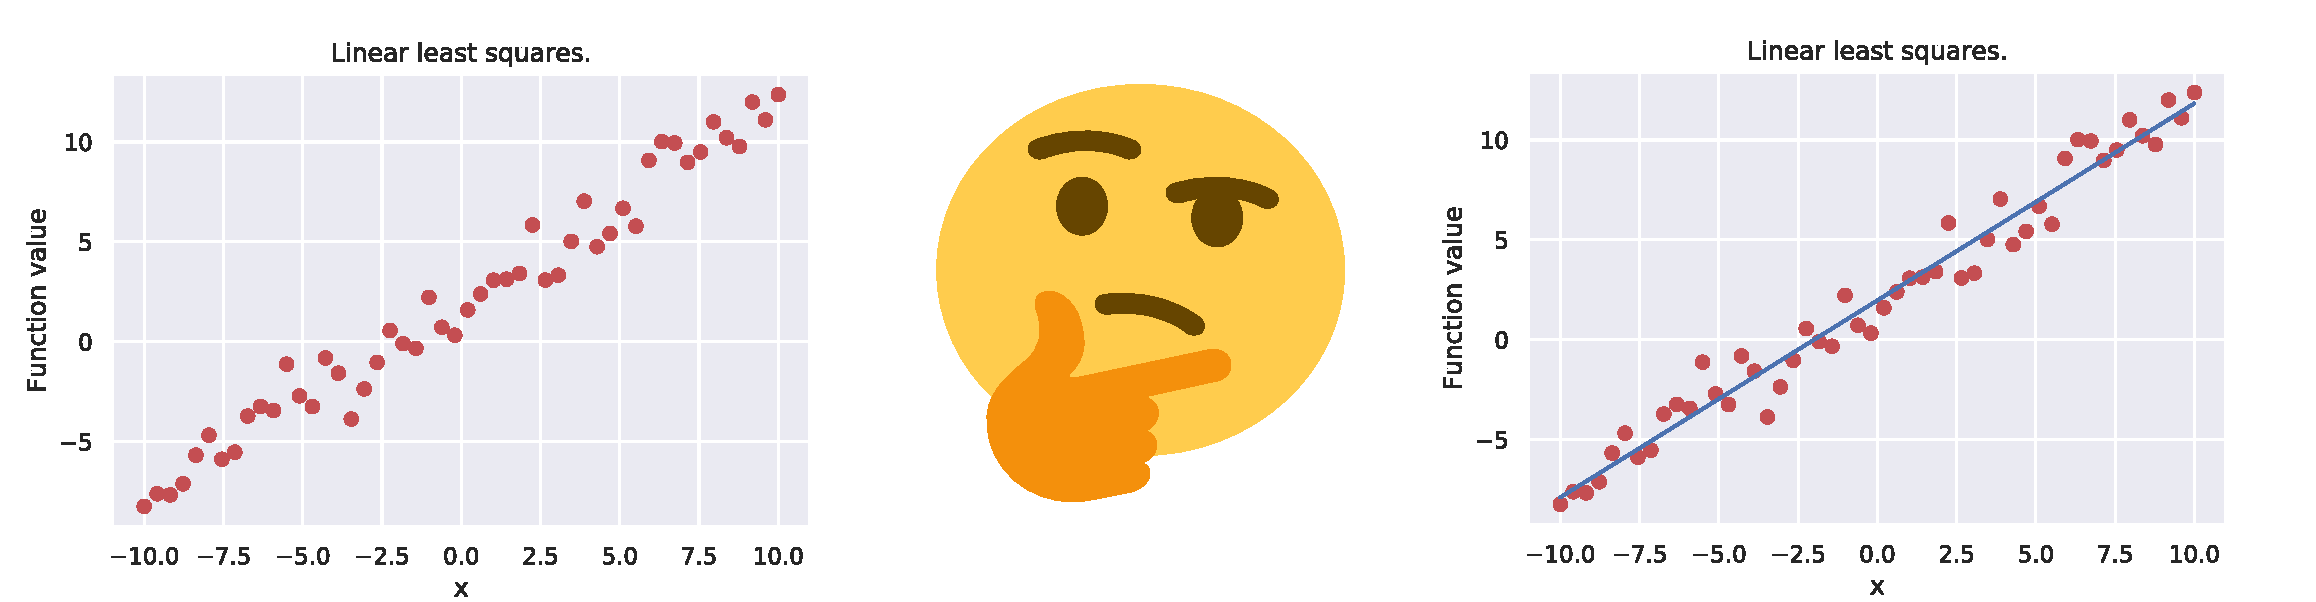
\includegraphics[width=0.75\linewidth,height=\textheight,keepaspectratio]{lls_idea.pdf}

}

\caption{Иллюстрация}

\end{figure}%

В задаче линейной регрессии у нас есть измерения
\(X \in \mathbb{R}^{m \times n}\) и \(y \in \mathbb{R}^{m}\) и мы ищем
вектор \(\theta \in \mathbb{R}^{n}\) такой, что \(X \theta\) близок к
\(y\). Близость определяется как сумма квадратов разностей: \[ 
\sum\limits_{i=1}^m (x_i^\top \theta - y_i)^2 = \|X \theta - y\|^2_2 \to \min_{\theta \in \mathbb{R}^{n}}
\] Например, рассмотрим набор данных, содержащий \(m\) пользователей,
каждый из которых представлен \(n\) признаками. Каждая строка
\(x_i^\top\) матрицы признаков \(X\) соответствует признакам
пользователя \(i\), а соответствующий элемент \(y_i\) вектора откликов
\(y\) представляет собой измеряемую величину, которую мы хотим
предсказать на основе \(x_i^\top\), например, расходы на рекламу.
Предсказание значения осуществляется по формуле \(x_i^\top \theta\).

\begin{enumerate}
\def\labelenumi{\arabic{enumi}.}
\tightlist
\item
  Является ли эта задача выпуклой? Сильно выпуклой?
\item
  Что вы думаете о сходимости градиентного спуска для этой задачи?
\end{enumerate}

\subsection{\texorpdfstring{\(l_2\)-регуляризованный метод наименьших
квадратов}{l\_2-регуляризованный метод наименьших квадратов}}\label{l_2-ux440ux435ux433ux443ux43bux44fux440ux438ux437ux43eux432ux430ux43dux43dux44bux439-ux43cux435ux442ux43eux434-ux43dux430ux438ux43cux435ux43dux44cux448ux438ux445-ux43aux432ux430ux434ux440ux430ux442ux43eux432}

В случае недоопределенной задачи может возникнуть желание восстановить
сильную выпуклость целевой функции, добавив \(l_2\)-штраф, также
известный как регуляризация Тихонова, \(l_2\)-регуляризация или
демпфирование весов. \[
\|X \theta - y\|^2_2 + \dfrac{\mu}{2} \|\theta\|^2_2\to \min_{\theta \in \mathbb{R}^{n}}
\] Примечание: С этой модификацией целевая функция снова становится
\(\mu\)-сильно выпуклой.

Посмотрите на
\href{https://colab.research.google.com/github/MerkulovDaniil/optim/blob/master/assets/Notebooks/l2_LLS.ipynb}{\faPython код}

\subsection{Наиболее важная разница между выпуклостью и сильной
выпуклостью}\label{ux43dux430ux438ux431ux43eux43bux435ux435-ux432ux430ux436ux43dux430ux44f-ux440ux430ux437ux43dux438ux446ux430-ux43cux435ux436ux434ux443-ux432ux44bux43fux443ux43aux43bux43eux441ux442ux44cux44e-ux438-ux441ux438ux43bux44cux43dux43eux439-ux432ux44bux43fux443ux43aux43bux43eux441ux442ux44cux44e}

\[
f(x) = \frac{1}{2m}\|A x - b\|^2_2 + \dfrac{\mu}{2} \|x\|^2_2\to \min_{x \in \mathbb{R}^{n}}, \quad A \in \mathbb{R}^{m \times n}, b \in \mathbb{R}^m
\]

\begin{figure}[H]

{\centering 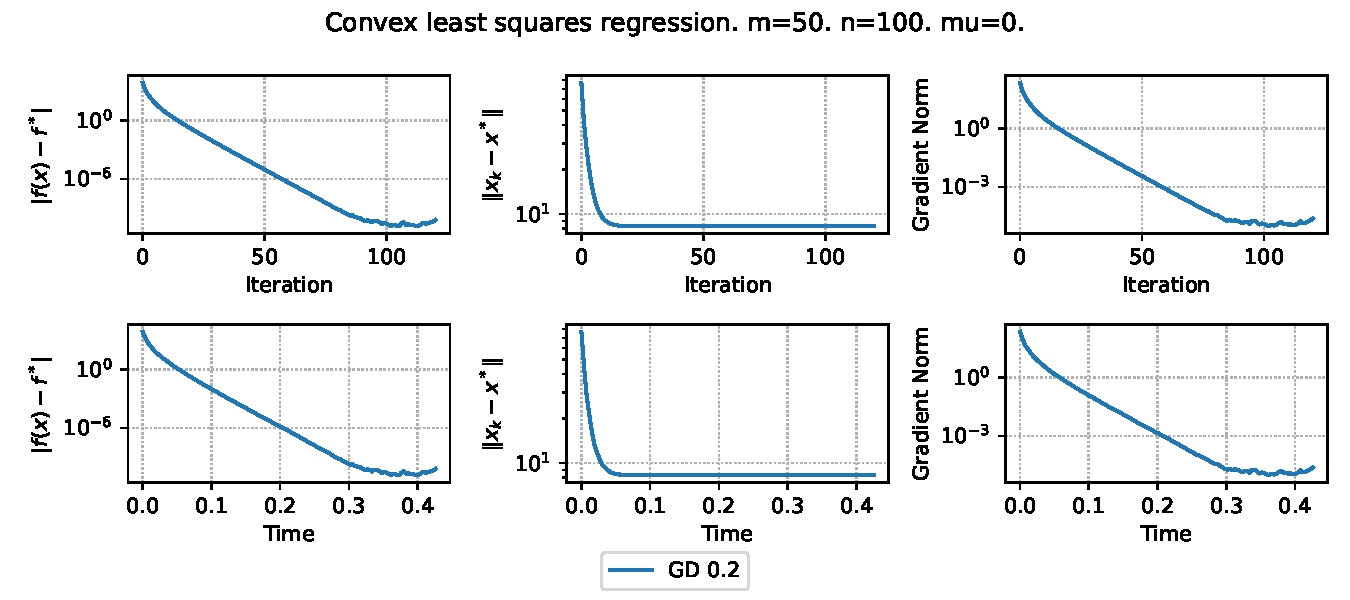
\includegraphics[width=0.85\linewidth,height=\textheight,keepaspectratio]{lls_convex.pdf}

}

\caption{Выпуклая задача не имеет сходимости по аргументу}

\end{figure}%

\[
f(x) = \frac{1}{2m}\|A x - b\|^2_2 + \dfrac{\mu}{2} \|x\|^2_2\to \min_{x \in \mathbb{R}^{n}}, \quad A \in \mathbb{R}^{m \times n}, b \in \mathbb{R}^m
\]

\begin{figure}[H]

{\centering 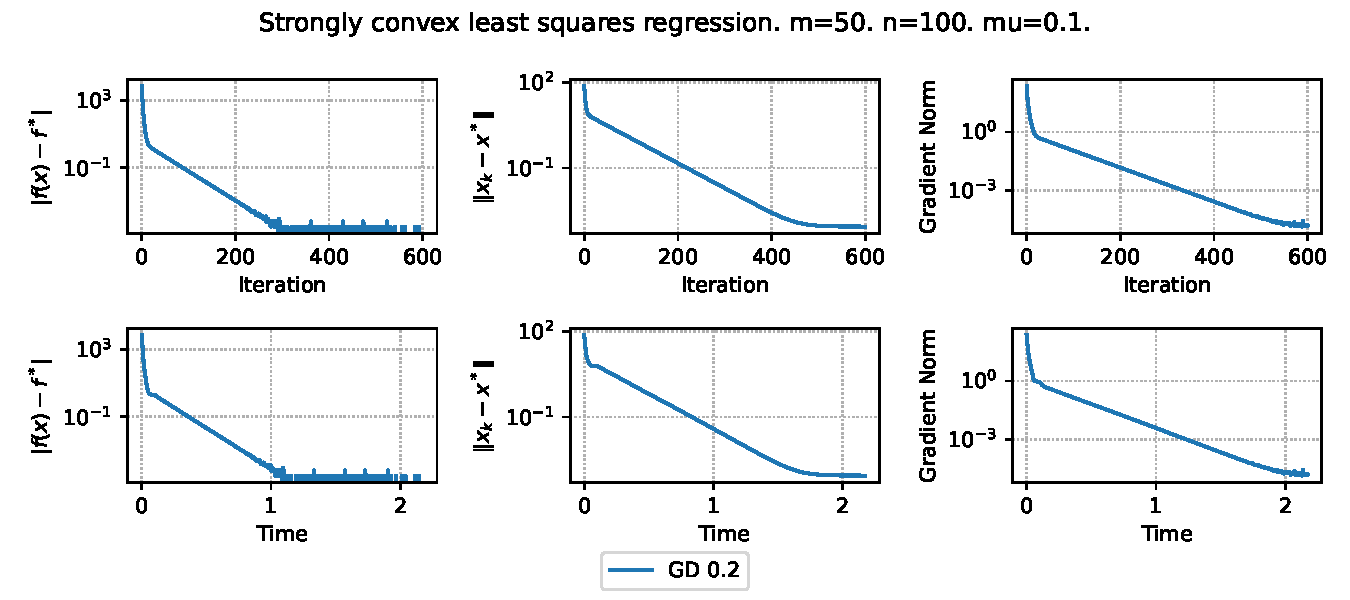
\includegraphics[width=0.85\linewidth,height=\textheight,keepaspectratio]{lls_convex_l2.pdf}

}

\caption{Но если добавить даже небольшую регуляризацию, вы гарантируете
сходимость по аргументу}

\end{figure}%

\[
f(x) = \frac{1}{2m}\|A x - b\|^2_2 + \dfrac{\mu}{2} \|x\|^2_2\to \min_{x \in \mathbb{R}^{n}}, \quad A \in \mathbb{R}^{m \times n}, b \in \mathbb{R}^m
\]

\begin{figure}[H]

{\centering 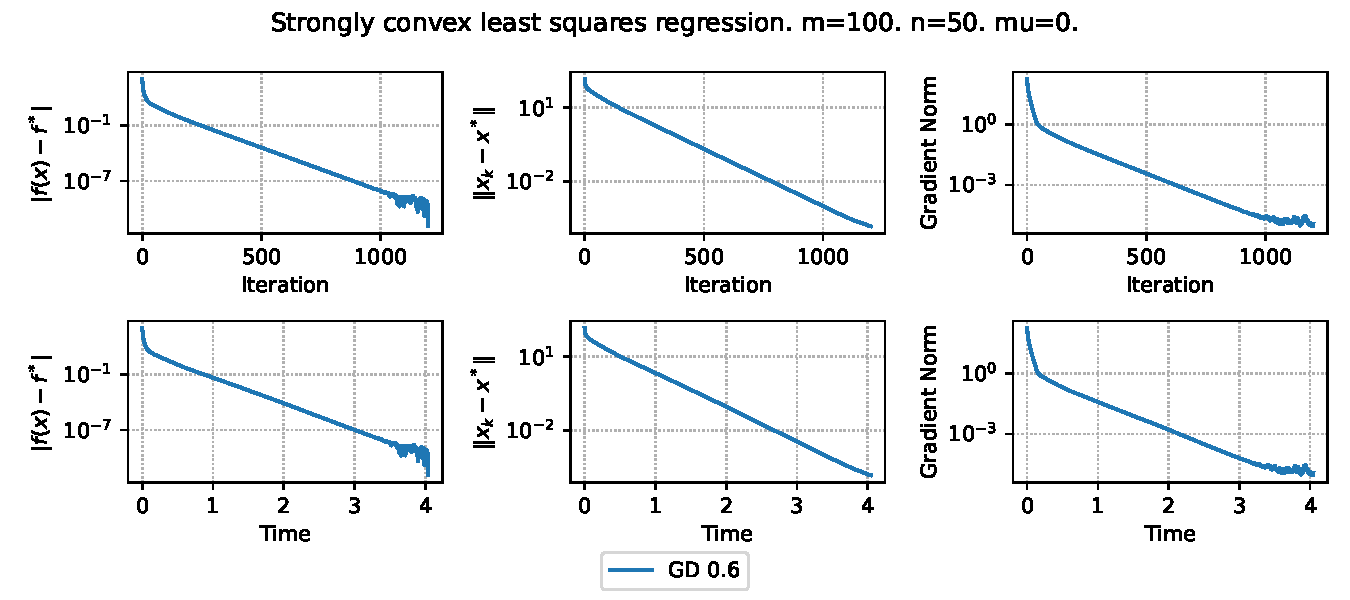
\includegraphics[width=0.85\linewidth,height=\textheight,keepaspectratio]{lls_strongly_convex.pdf}

}

\caption{Другой способ обеспечить сходимость в предыдущей задаче -
поменять местами значения размерности задачи}

\end{figure}%

\subsection{Для сходимости к решению с высокой точностью необходима
сильная выпуклость (или выполнение условия
Поляка-Лоясиевича).}\label{ux434ux43bux44f-ux441ux445ux43eux434ux438ux43cux43eux441ux442ux438-ux43a-ux440ux435ux448ux435ux43dux438ux44e-ux441-ux432ux44bux441ux43eux43aux43eux439-ux442ux43eux447ux43dux43eux441ux442ux44cux44e-ux43dux435ux43eux431ux445ux43eux434ux438ux43cux430-ux441ux438ux43bux44cux43dux430ux44f-ux432ux44bux43fux443ux43aux43bux43eux441ux442ux44c-ux438ux43bux438-ux432ux44bux43fux43eux43bux43dux435ux43dux438ux435-ux443ux441ux43bux43eux432ux438ux44f-ux43fux43eux43bux44fux43aux430-ux43bux43eux44fux441ux438ux435ux432ux438ux447ux430.}

\begin{figure}[H]

{\centering 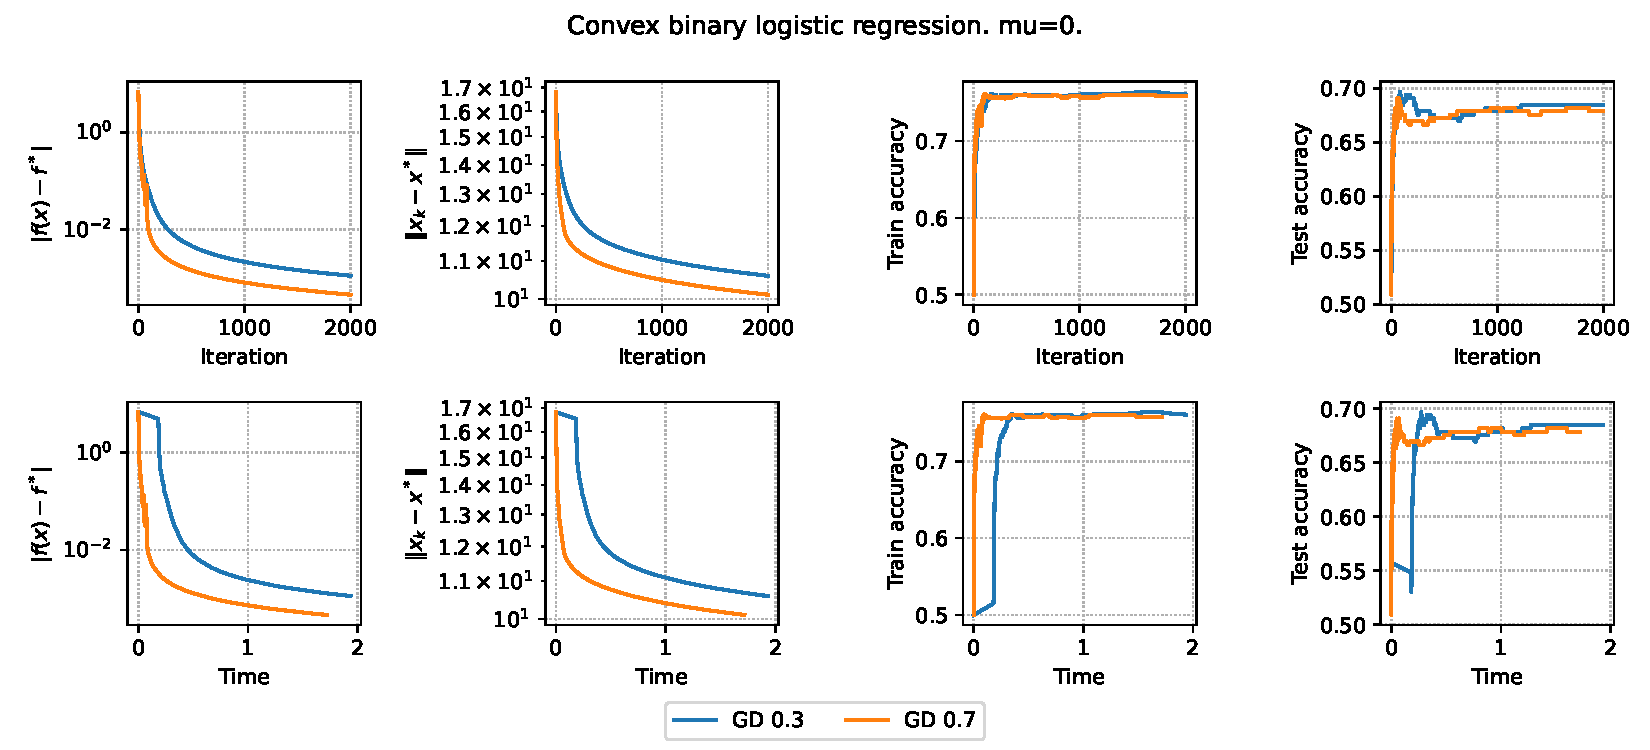
\includegraphics[width=0.85\linewidth,height=\textheight,keepaspectratio]{logreg_convex.pdf}

}

\caption{Лишь небольшая точность может быть достигнута с сублинейной
сходимостью}

\end{figure}%

\begin{figure}[H]

{\centering 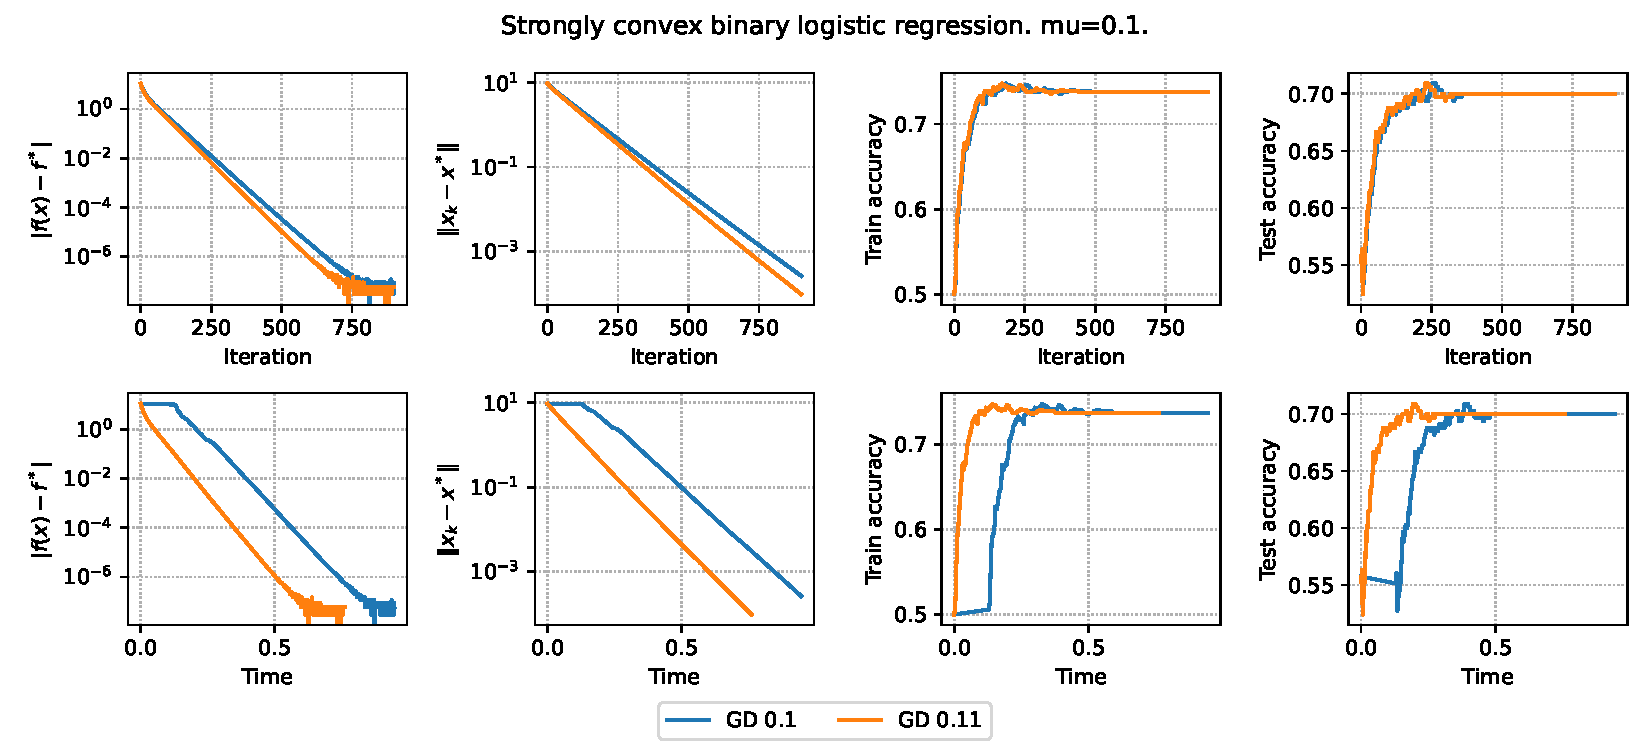
\includegraphics[width=0.85\linewidth,height=\textheight,keepaspectratio]{logreg_strongly_convex.pdf}

}

\caption{Сильная выпуклость обеспечивает линейную сходимость}

\end{figure}%

\subsection[Любой локальный минимум является глобальным минимумом для
глубоких линейных сетей ]{\texorpdfstring{Любой локальный минимум
является глобальным минимумом для глубоких линейных сетей
\footnote{\href{https://arxiv.org/abs/1707.02444}{Глобальные условия
  оптимальности для глубоких нейронных сетей}}}{Любой локальный минимум является глобальным минимумом для глубоких линейных сетей }}\label{ux43bux44eux431ux43eux439-ux43bux43eux43aux430ux43bux44cux43dux44bux439-ux43cux438ux43dux438ux43cux443ux43c-ux44fux432ux43bux44fux435ux442ux441ux44f-ux433ux43bux43eux431ux430ux43bux44cux43dux44bux43c-ux43cux438ux43dux438ux43cux443ux43cux43eux43c-ux434ux43bux44f-ux433ux43bux443ux431ux43eux43aux438ux445-ux43bux438ux43dux435ux439ux43dux44bux445-ux441ux435ux442ux435ux439}

Рассмотрим следующую задачу оптимизации: \[
\min_{W_1, \dots, W_L} L(W_1, \dots, W_L) = \frac{1}{2} \|W_L W_{L-1} \cdots W_1 X - Y\|_F^2,
\] где

\textbf{\(X \in \mathbb{R}^{d_x \times n}\)} - матрица данных/входных
данных,

\textbf{\(Y \in \mathbb{R}^{d_y \times n}\)} - матрица меток/выходных
данных.

\begin{tcolorbox}[enhanced jigsaw, colframe=quarto-callout-color-frame, titlerule=0mm, coltitle=black, toprule=.15mm, colback=white, leftrule=.75mm, bottomtitle=1mm, toptitle=1mm, colbacktitle=quarto-callout-color!10!white, breakable, opacityback=0, bottomrule=.15mm, left=2mm, opacitybacktitle=0.6, title=\textcolor{quarto-callout-color}{\faInfo}\hspace{0.5em}{Theorem}, rightrule=.15mm, arc=.35mm]

Пусть \(k = \min(d_x, d_y)\) - ``ширина'' сети, и определим \[
V = \{ (W_1, \dots, W_L) \mid \operatorname{rank}(\Pi_i W_i) = k \}.
\] Тогда каждая критическая точка \(L(W)\) в \(V\) является глобальным
минимумом, в то время как каждая критическая точка в дополнении \(V^c\)
является седловой точкой.

\end{tcolorbox}

\section{Задачи}\label{ux437ux430ux434ux430ux447ux438}

\begin{enumerate}
\def\labelenumi{\arabic{enumi}.}
\item
  Докажите, что шар в \(\mathbb{R}^n\) (т.е. множество
  \(\{ \mathbf{x} \mid \Vert \mathbf{x} - \mathbf{x}_c \Vert \leq r \}\))
  - является выпуклым.
\item
  Является ли полоса
  \(\{x \in \mathbb{R}^n \mid \alpha \leq a^\top x \leq \beta \}\)
  выпуклой?
\item
  Пусть \(S\) такое, что
  \(\forall x,y \in S \to \frac{1}{2}(x+y) \in S\). Является ли это
  множество выпуклым?
\item
  Является ли множество \(S = \{x \; | \; x + S_2 \subseteq S_1\}\), где
  \(S_1,S_2 \subseteq \mathbb{R}^n\) с выпуклым \(S_1\), выпуклым?
\item
  Является ли множество \(S = \{x \; | \; x + S_2 \subseteq S_1\}\), где
  \(S_1,S_2 \subseteq \mathbb{R}^n\) с выпуклым \(S_1\), выпуклым?
\end{enumerate}

\section{Задачи на
дом}\label{ux437ux430ux434ux430ux447ux438-ux43dux430-ux434ux43eux43c}

\begin{enumerate}
\def\labelenumi{\arabic{enumi}.}
\item
  {[}10 points{]} Докажите, что эта функция выпукла: \[
   f(x, y, z) = z \log \left(e^{\frac{x}{z}} + e^{\frac{y}{z}}\right) + (z - 2)^2 + e^{\frac{1}{x + y}}
   \] где функция \(f : \mathbb{R}^3 \to \mathbb{R}\) имеет область
  определения, определенную как: \[
   \text{dom } f = \{ (x, y, z) \in \mathbb{R}^3 : x + y > 0, \, z > 0 \}.
   \]
\item
  {[}5 points{]} Центр масс тела является важным понятием в физике
  (механике). Для системы материальных точек с массами \(m_i\) и
  координатами \(x_i\), центр масс определяется как: \[
   x_c = \frac{\sum_{i=1}^k m_i x_i}{\sum_{i=1}^k m_i}
   \] Центр масс тела не всегда лежит внутри тела. Например, центр масс
  бублика находится в его отверстии. Докажите, что центр масс системы
  материальных точек лежит в выпуклой оболочке множества этих точек.
\item
  {[}8 points{]} Докажите, что
  \(\mathbf{conv}\{xx^\top: x \in \mathbb{R}^n, \Vert x\Vert  = 1\} = \{A \in \mathbb{S}^n_+: \text{tr}(A) = 1\}\).
\item
  {[}5 points{]} Докажите, что множество
  \(\{x \in \mathbb{R}^2 \mid e^{x_1}\le x_2\}\) является выпуклым.
\item
  {[}8 points{]} Рассмотрим функцию \(f(x) = x^d\), где
  \(x \in \mathbb{R}_{+}\). Заполните следующую таблицу ✅ или ❎.
  Объясните свои ответы (с доказательствами).

  \begin{longtable}[]{@{}ccccc@{}}
  \toprule\noalign{}
  \(d\) & Выпуклая & Вогнутая & Строго выпуклая & \(\mu\)-сильно
  выпуклая \\
  \midrule\noalign{}
  \endhead
  \bottomrule\noalign{}
  \endlastfoot
  \(-2, x \in \mathbb{R}_{++}\) & & & & \\
  \(-1, x \in \mathbb{R}_{++}\) & & & & \\
  \(0\) & & & & \\
  \(0.5\) & & & & \\
  \(1\) & & & & \\
  \(\in (1; 2)\) & & & & \\
  \(2\) & & & & \\
  \(> 2\) & & & & \\
  \end{longtable}
\item
  {[}6 points{]} Докажите, что функция энтропии, определенная как \[
   f(x) = -\sum_{i=1}^n x_i \log(x_i),
   \] с \(\text{dom}(f) = \{x \in \R^n_{++} : \sum_{i=1}^n x_i = 1\}\),
  является строго вогнутой.
\item
  {[}8 points{]} Докажите, что максимум выпуклой функции \(f\) над
  многогранником\(P = \text{conv}\{v_1, \ldots, v_k\}\) достигается в
  одной из его вершин, т.е. \[
   \sup_{x \in P} f(x) = \max_{i=1, \ldots, k} f(v_i).
   \]

  Более сильное утверждение: максимум выпуклой функции над замкнутым
  ограниченным выпуклым множеством достигается в крайней точке, т.е.
  точке в множестве, которая не является выпуклой комбинацией любой
  другой точки в множестве. (вы не должны его доказывать).
  \emph{Подсказка:} Предположите, что утверждение неверно, и используйте
  неравенство Йенсена.
\item
  {[}6 points{]} Докажите, что два определения \(\mu\)-сильно выпуклых
  функций эквивалентны:

  \begin{enumerate}
  \def\labelenumii{\arabic{enumii}.}
  \item
    \(f(x)\) является \(\mu\)-сильно выпуклой \(\iff\) для любых
    \(x_1, x_2 \in S\) и \(0 \le \lambda \le 1\) для некоторого
    \(\mu > 0\): \[
     f(\lambda x_1 + (1 - \lambda)x_2) \le \lambda f(x_1) + (1 - \lambda)f(x_2) - \frac{\mu}{2} \lambda (1 - \lambda)\|x_1 - x_2\|^2
     \]
  \item
    \(f(x)\) является \(\mu\)-сильно выпуклой \(\iff\) если существует
    \(\mu>0\) такое, что функция \(f(x) - \dfrac{\mu}{2}\Vert x\Vert^2\)
    является выпуклой.
  \end{enumerate}
\end{enumerate}




\end{document}
